\documentclass[pdftex,12pt,a4paper]{article}

\usepackage[top=3cm, bottom=3cm, left=3.5cm, right=3cm]{geometry}

% graphics images
\usepackage[pdftex]{graphicx}

% 1.5 line spacing
\usepackage{setspace}
\onehalfspacing

% maths symbols
\usepackage{amsmath}

% table package
\usepackage{multirow}
\usepackage{tabu}
\usepackage{tabularx}
\usepackage{pbox}

% citation style
\usepackage{listings}
\usepackage{color}

\usepackage{multirow}
\usepackage{algorithm}
\usepackage{algpseudocode}
\usepackage{algorithmicx}
\algdef{SE}[DOWHILE]{Do}{doWhile}{\algorithmicdo}[1]{\algorithmicwhile\ #1}%


\NeedsTeXFormat{LaTeX2e}
% \ProvidesPackage{math}
% \RequirePackage{amsmath,amsthm,amsfonts,amssymb}

% SVM
\providecommand{\pd}[2]{\frac{\partial #1}{\partial #2}}

\providecommand{\abs}[1]{\lvert #1 \rvert}
\providecommand{\norm}[1]{\lVert #1 \rVert}
\providecommand{\inprod}[2]{\langle{#1},{#2}\rangle}
\providecommand{\avg}[1]{\langle#1\rangle}

\providecommand{\set}[1]{\{#1\}}

\DeclareMathOperator{\Prob}{P}
\DeclareMathOperator{\E}{E}
\DeclareMathOperator{\tr}{tr}
\DeclareMathOperator{\var}{var}
\DeclareMathOperator{\sign}{sign}
% SVM

\newcommand{\argmax}[1]{\underset{#1}{\operatorname{arg}\,\operatorname{max}}\;}

\definecolor{dkgreen}{rgb}{0,0.6,0}
\definecolor{gray}{rgb}{0.5,0.5,0.5}
\definecolor{mauve}{rgb}{0.58,0,0.82}
\lstset{frame=tb,
  language=Java,
  aboveskip=3mm,
  belowskip=3mm,
  showstringspaces=false,
  columns=flexible,
  basicstyle={\small\ttfamily},
  numbers=none,
  numberstyle=\tiny\color{gray},
  keywordstyle=\color{blue},
  commentstyle=\color{dkgreen},
  stringstyle=\color{mauve},
  breaklines=true,
  breakatwhitespace=true
  tabsize=3
}

\newcommand{\head}[1]{\textnormal{\textbf{#1}}}
\newcommand{\HRule}{\rule{\linewidth}{0.5mm}}


\usepackage[font={it}]{caption}

\begin{document}
% \tableofcontents
\newpage
% \section {Introduction}
Nowadays, with the development of technology, digital cameras and mobile phones with cameras are becoming more and more common. As a result, the number of videos are increasing exponentially. According to Youtube statistics, 100 hours of videos are uploaded every minute, and over 6 billion hours of videos are watched each month in Youtube. Due to such a large number of videos, it is urgent and important to develop effective and robust approach to index and retrieve videos. Also, because of the large number of videos, it is costly to rely on human power to recognize videos. Thus, one direction is to recognize videos by leveraging machine intelligence. The general way is to use a set of training videos with labels to build classifiers. Afterward, these classifiers could be used to predict labels for new coming videos. However, in order to build a robust classifier, there is a lot of work to do. \\

\noindent In this final year project, various approaches are studied and implemented to recognize videos. This project starts with image recognition because the data size of images is much smaller compared with videos. To represent images, SIFT features \cite{lowe2004distinctive} are extracted from images, the features of each image are converted into a histogram based on visual vocabulary built through clustering algorithm using spatial pyramid matching \cite{lazebnik2006beyond}. Then such representations are input into machine learning classification methods including SVM and KNN for recognition. Furthermore, to better calculate image-to-image distance, earth mover's distance (EMD) \cite{rubner2000earth} is incorporated, and the recognition accuracy demonstrates the effectiveness of EMD. Also, a method to identify representative images from a cluster of images is introduced, and this method is later on use to compress videos to remove redundant frames. This project then moves to video recognition, in which two types of representations are adopted to represent videos. The first one is the famous bag of words model which treats each video as multiple frames and represents each video as a stack of histograms \cite{duan2012visual} where each histogram represents a frame in that video. Also, in the second representation, each video is treated as a bag of SIFT features \cite{zhou2008sift}, and specialized Gaussian Mixture Models (GMM) are built on this bag to represent this video. Before building specialized GMM, a global GMM is first built on SIFT features of all training videos. Due to two different representations of videos, two different distance calculations are used. Furthermore, concept attribute \cite{liu2013video}, which models each video as a vector of scores of semantic concepts, is also studied and implemented. based on the performance, it shows that such short vector representation still retains comparable discriminable power compared with original representations of videos. This is not the end of story. Promising domain adaptations methods \cite{duan2012visual, duan2009domain, yang2007cross, daume2007frustratingly}, which leverage labelled samples from other domains, are also researched. Feature Replication, Adaptive SVM, Domain Transfer SVM and Adaptive Multiple Kernel Learning are implemented in Python and improve the performance of recognition from the original $44.33\%$ to as high as $61.40\%$ using the metric of mean average precision. Lastly, a web based demo system is implemented to present the work in this project. \\

\noindent The rest of this report is organized as follows: firstly, literature review is presented followed by the section of details on image recognition. Secondly, the section of video recognition, which introduces Aligned Space-Time Pyramid Matching and Specialized Gaussian Mixture Models, is presented. Thirdly, four domain adaptations methods are talked about followed by the section of comprehensive experiments. Next, the design of web-based demo system is briefly introduced. Finally, this report ends with the section of conclusion. 
% \section{Literature review}
% \section {Image Recognition}
Image recognition is a very interesting topic in computer vision and pattern recognition, and the goal is to recognize different classes in images. For instance, there are trees, people, sun, moon and buildings in different images. Human can easily distinguish different classes among a set of images. However, machines are not good at such tasks. For many years, a lot of researchers are working on this topic and have achieved significant results.\\

\noindent So far, a very good framework to recognize images is the so-called {\em bag of words} model, which generalizes from natural language processing (NLP). In NLP, bag of words basically aims to represent an article using histogram of word frequencies. Following this idea, in image recognition, an image is also represented as a histogram of visual words, and these visual words normally come from centroids generated from clustering algorithms. Later on, such representations of images are used to build up generic machine learning models, and the accuracy is quite impressive. During recognition phase, the most critical process is to calculate image-to-image distance. One direct way is the Euclidean distance. But a better way to calculate distance is called as Earth Mover's Distance \cite{rubner2000earth}, which finds the best matches between image parts and produces a more accurate distance. \\

\noindent In the following of this section, an image recognition framework consisting of 4 steps is first introduced. Secondly, Earth Mover's distance and its applications in image recognition is talked about. Lastly, the method to identify duplicates in a cluster of images used in this project are presented, and this method is going to be applied in video recognition to show the effectiveness of Earth Mover's distance.

\subsection{Framework Description}

Generally, there are 4 below steps to go:

\subsubsection{Extract SIFT features from each image}
It is almost impossible to directly rely on pixel data of images to perform recognition tasks, and the main reason is because such pixel data does not possess much discriminative power. Therefore, other approaches to represent images are needed. One approach is to extract features from images and use those features to represent images compactly. There are generally two categories of features: global features and local features. As the name stated, global features encode a whole image based on the overall distribution of color, texture, or edge information. Some popular global features include color histogram and Gabor texture \cite{manjunath1996texture}. On the other hand, local features refer to features extracted from local patches (or interest points). There are two steps involved in extracting local features: detection and description. Detection refers to localizing interest points in images. Among popular detection algorithms, the most widely used is Difference-of-Gaussian (DOG) \cite{lowe2004distinctive} introduced by David Lowe, which detects blob regions where the centroids differs from their neighbors. Other popular detectors include Harris-Laplace \cite{lindeberg1998feature}, Hessian \cite{mikolajczyk2004scale}, etc. The next stage is description which aims to describe those located interest points in meaningful manners such that this descriptor is invariant to scale, viewpoint, rotation and illumination changes. There are lots of descriptors that have been designed over years. The best known shall be Scale Invariant Feature Transform (SIFT) \cite{lowe2004distinctive}, which concatenates histograms of gradient orientation around interest points. Other descriptors include Histogram of oriented gradients (HOG) \cite{dalal2005histograms}, Local binary pattern (LBP) \cite{ojala2002multiresolution}, etc. Given the robustness of SIFT shown in various literatures \cite{duan2012visual,zhou2008sift,lazebnik2006beyond, lowe2004distinctive}, SIFT is chosen to be the feature to be extracted from images through the whole period of this project.\\

\noindent Now it's time to briefly elaborate details about SIFT. There are two steps when performing extracting SIFT features. The first step is to identify interest points, and the criteria is based on {\em difference-of-Gaussian functions}:
\begin{equation}
D(x, y, \sigma) = (G(x, y, k\sigma) - G(x, y, \sigma)) * I(x, y)
\end{equation}

\noindent where $G$ is the Gaussian 2D kernel, $I(x, y)$ is an input image and $k$ is a constant multiplicative factor which separates two nearby scales. After computing $D(x, y, \sigma)$ for all sample points, those sample points with local maxima and minima of $D(x, y, \sigma)$ compared with their neighbors are selected to be interest points. In order to better localize interest points, these candidate locations are filtered to remove unstable points based on criteria including low contrast and edge response. Please refer to the paper \cite{lowe2004distinctive} for details on removing unstable points. The next step is to compute a descriptor based on those interest points located in previous step. For each interest point, a descriptor is created by first computing the gradient magnitude and orientation in a grid of subregions around that specific interest point. These gradient orientations are then accumulated into orientation histograms. Finally, these histograms are concatenated to form a descriptor vector. The recommended setting uses $4 \times 4$ subregions with 8 bin histogram, which results in a 128 bin histograms ($4 \times 4 \times 8 = 128$). Figure 1 below demonstrates the whole process to construct SIFT descriptor. \\

\begin{figure}[!ht]
\centering
  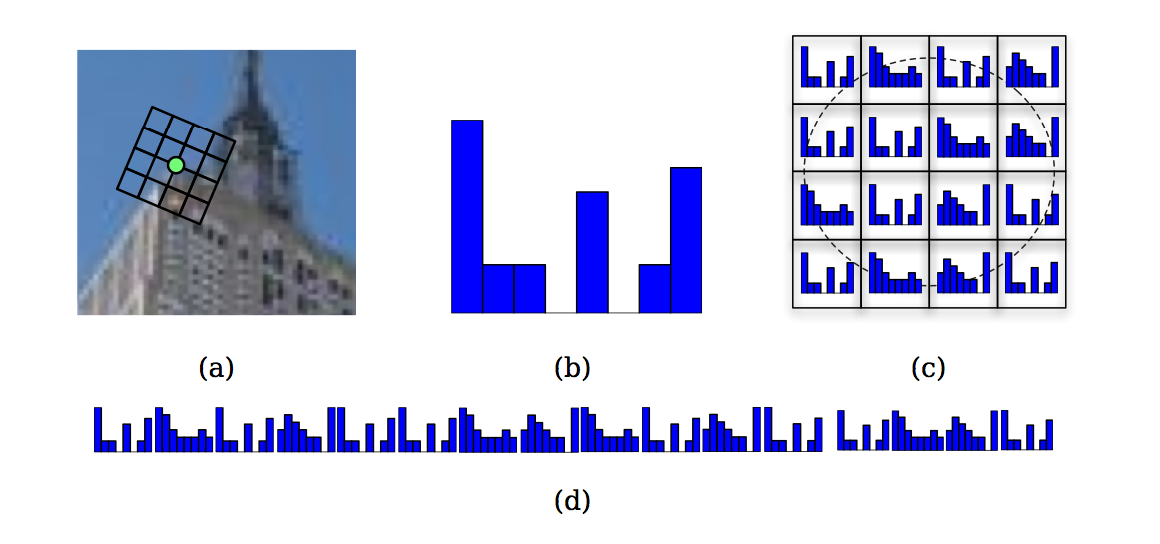
\includegraphics[width=1\textwidth]{./SIFT_Descriptor.png}
\caption{SIFT descriptor \cite{solem2012programming} (a) a frame with $4 \times 4$ subregions around an interest point. (b) an 8 bin histogram over the direction of gradient in one subregion. (c) all histograms in their respective subregions. (d) all 16 histograms are concatenated to form a 128 ($16 \times 8$) dimensional vector.}
\end{figure}

\noindent For simplicity, an open source library VLFEAT \cite{vedaldi08vlfeat} is adopted to extract SIFT from images. A typical image of size $200 \times 200$ normally produces around 800 SIFT features.  

\subsubsection{Build up visual vocabulary from features of training set}
Although SIFT features have been extracted, these 128 dimensional raw features are still not an ideal representation because of limitations including the curse of dimensionality. Thus, a visual vocabulary is needed to map high dimensional descriptors to words by quantizing the feature space. Commonly, vocabulary is built through applying K-Means \cite{lloyd1982least} clustering algorithm on available features, and the final centroids output by K-Means are treated as representative words. The basic K-means algorithm goes as below:

\begin{algorithm}
  \caption{Basic K-means Algorithm}
  \begin {algorithmic}[1]
  \State Randomly select K points as the initial centroids
  \Do 
    \State Form K clusters by assigning all points to their closest centroids.
    \State Recompute the centroid of each cluster
  \doWhile Centroids are changed
  \end{algorithmic}
\end{algorithm}

\noindent Based on the above algorithm, it is easy to see that the time complexity is $O(n*K*I*d)$, where $n$ is the number of points, $K$ is the number of clusters, $I$ is the number of iterations and $d$ is the number of dimensions. This classical K-means algorithm works fine for small data sets but is very expensive for large data sets. Later on, vocabulary is also needed for video recognition where the number of features is nearly 0.4 million after sampling. By noticing that the available computational resource is limited, it is not affordable to apply classical K-Means on large data sets. Therefore, a better method is needed to build up vocabularies.  Mini-Batch K-Means \cite{sculley2010web}, a variant of KMeans algorithm which uses mini-batches to reduce the computation time, is a good alternative. In contrast to other algorithms which reduce the convergence time of k-means, mini-batch k-means produces results that are generally only slightly worse than the standard algorithm. The details about mini-batch k-means are presented as follows:

\begin{algorithm}
  \caption{Mini-batch K-Means}
  \begin{algorithmic}[1]
  \State Given: $k$, mini-batch size $b$, iteration $t$, data set $X$
  \State Initialize each $c \in C$ with an $x$ picked randomly from $X$
  \State $v \gets 0$
  \For {$i = 1$ to $t$}
  \State $M \gets b$ examples picked randomly from $X$
  
  \For {$x \in M$}
  \State $d[x] \gets f(C, x)$ \Comment{Cache the nearest center to $x$}
  \EndFor

  \For {$x \in M$}
  \State $c \gets d[x]$ \Comment{Get cached center for this $x$}
  \State $v[c] \gets v[c] + 1$ \Comment{Update per-center counts}
  \State $\eta \gets \frac{1}{v[c]}$ \Comment{Get per-center learning rate}
  \State $c \gets (1 - \eta)c + \eta x$ \Comment{Take gradient step}
  \EndFor
  
  \EndFor
  \end{algorithmic}
\end{algorithm}

\noindent Once this vocabulary is built, a histogram whose length equals to the size of vocabulary is built for each image. Afterward, features of images are examined to construct their histograms. For each SIFT feature, the nearest word to this feature is found, and the bin representing the found word is increased by one. After finishing examining all features, a histogram is constructed and is used to represent the respective image. As a result, all images are transformed from pixels to fixed length histograms. In image recognition experiments, the number of centroids is set to be 300 when performing Mini-Batch K-Means. Thus, all images are converted into 300 dimensional histograms. 

\subsubsection{Construct a pyramid of three levels for each image}
Now that histograms for images are built, these histograms could be put into machine learning models including K Nearest Neighbor and Support Vector Machine for recognition. However, this is not the end of story. To enable more discriminative power, Grauman and Darrell \cite{grauman2005pyramid} proposed {\em pyramid matching} in 2005 to find an approximate correspondence between 2 sets of data. The basic idea is to map sets of features to multi-resolution histograms, and then compare the histograms with a weighted histogram intersection measure in order to better approximate the similarity of best partial matching. As reported in the paper \cite{grauman2005pyramid}, this pyramid match kernel produces much better recognition results for similar running time. \\

\noindent Though {\em pyramid matching} fuses information from multiple levels built on different resolutions, this method ignores spatial information because features are matched without any order. To partially address this problem, in the following year, Lazebnik introduced spatial pyramid matching \cite{lazebnik2006beyond}. Unlike pyramid matching which varies histogram matching resolution, spatial pyramid matching varies the spatial resolution at which they are aggregated. Figure 2 below demonstrates the case when there are three levels in spatial pyramid matching. The three levels are presented from the left to right. Level 0 is simply a standard bag of features which treats the whole image as a whole. For level 1, this image is divided equally into 4 parts, each part contributes to one histogram built on the same vocabulary. Furthermore, level 2 is the case when image is divided into 16 parts which results in 16 different histograms. Finally, all these histograms are concatenated with appropriate weights to form a ``long'' histogram with dimensionality as $M\sum_{l=0}^{L}4^{l}$, where $M$ is the size of vocabulary and $L$ equals to total number of levels $ - 1$. For instance, the vocabulary size used in experiments is 300. Thus, the number of dimensions is 1500 for two-level spatial pyramid and 6300 for three-level spatial pyramid. Additionally, the weights for histograms at different levels are listed below:

\begin{equation}
 weight(l) = \left\{ 
\begin{array}{l l}
  \frac{1}{2^L} & \quad \text{$if \ l = 0$ }\\
  \frac{1}{2^{L-l+1}} & \quad \text{$Otherwise$}
\end{array} \right.
\end{equation}

\noindent For example, as shown in Figure 2, weights for three levels histograms are $\frac{1}{4}$, $\frac{1}{4}$ and $\frac{1}{2}$, respectively. It is easy to see that such weighting scheme tends to penalize matches found in larger cells, and the reason why it makes sense is because larger cells allow more dissimilar features. 

\begin{figure}[!ht]
\centering
  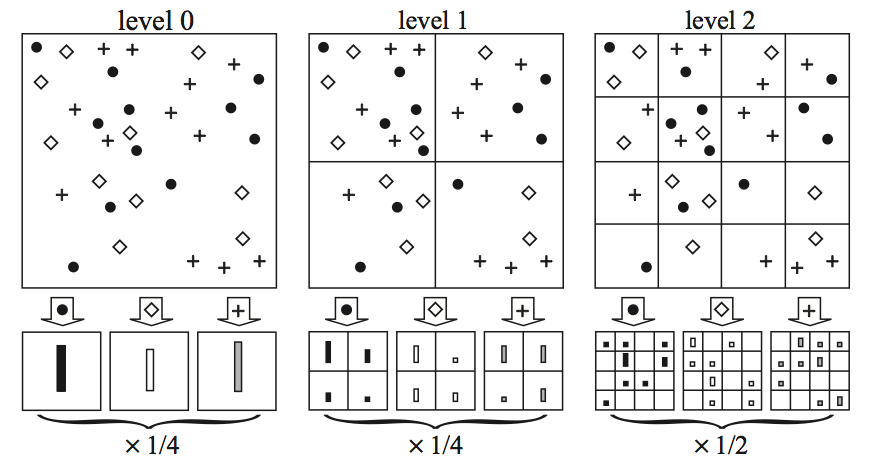
\includegraphics[width=1\textwidth]{./SpatialPyramidMatch.png}
\caption{Example to construct a three-level pyramid \cite{lazebnik2006beyond}. At top, images are divided at three different levels of resolution. Next, the count to each feature is calculated for each spatial bin. Finally, each histogram is weighted according to equation (2)}
\end{figure}

\subsubsection{Classify based on above representations}
In machine learning, classification refers to the problem of identifying to which category a new observation belongs, on the basis of training data set. Generally, machine learning builds a model which fits the training data set. Afterward, this model to use to recognize new data set. There are many classification methods including K-nearest neighbors (KNN), support vector machine (SVM), decision tree, etc. In this project, KNN and SVM are incorporated into the recognition system, and details about these two kinds of classification methods will be presented in following paragraphs. 

  \paragraph{K-nearest neighbor (KNN)} 
  K-nearest neighbor is considered as a lazy learning algorithm. This is because it does not attempt to construct a general internal model, but just store all instances of the training data. Once a test case is input, KNN retrieves the nearest $K (K>0)$ neighbors to this test case from training data, and the predicted label is computed based on labels of neighbors in a majority vote manner. In other words, the predicted label of a test case is chosen to be the most representative label among $K$ nearest neighbors. For example, Figure 3 shows how to predict label for $x_{q}$ when $K$ is set to be 5. Among 5 neighbors of $x_{q}$, three are negative while the left two are positive. Therefore, $x_{q}$ is predicted to be within negative class based on majority vote. 

  \begin{figure}[!ht]
  \centering
    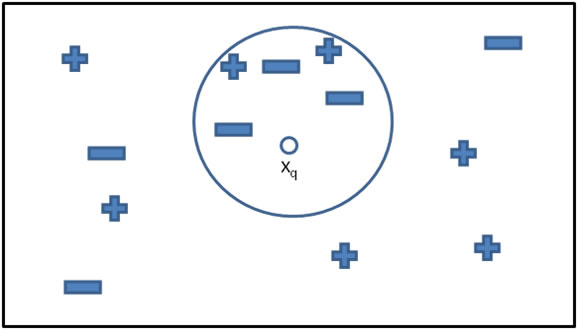
\includegraphics[scale=0.5]{./knn.jpg}
  \caption{A case of k nearest neighbor. Among 5 neighbors of $x_{q}$, three are negative while the other two are positive. As a result, the label of $x_{q}$ is predicted to be negative.}
  \end{figure}

  \paragraph{Support vector machine (SVM)}
  Support Vector Machine was introduced in COLT-92 by Boser, Guyon \& Vapnik \cite{boser1992training} and became rather popular since then. This is a well motivated algorithm which is developed from statistical learning theory since 1960s. It has been successfully applied into many fields (bioinformatics, text, image recognition, ...) and is currently the most popular classifier in event recognition systems \cite{jiang2012high}. \\

  \noindent SVM starts with the problem of finding the optimal separating hyperplane which separates a linearly separable dataset: $${(x_{1}, y_{1}), (x_{2}, y_{2}), ..., (x_{n}, y_{n})}$$ where $x \in R^{D}$ and $y \in  \{ -1, +1 \}$. An example is presented in Figure 4. Black solid circle represents one class while the while circle represents another class. The solid line $\mathbf{w} \mathbf{x} + b = 0$ is the optimal hyperplane, and the data points on $\mathbf{w} \mathbf{x} + b = 1$ and $\mathbf{w} \mathbf{x} + b = -1$ are called are {\em support vectors}. It is not difficult to see that the distances from support vectors to optimal hyperplane  are maximized. Therefore, the finding of optimal hyperplane is transformed into an optimization problem:
  \begin{eqnarray}
  & \text{minimize} \quad J(w) = \frac{1}{2} \norm{w}^2 \nonumber \\
  & \text{subject to} \quad y_i (w^{T} x_i + b) \ge 1 \quad \forall i
  \end{eqnarray}
  
  \begin{figure}[!ht]
  \centering
    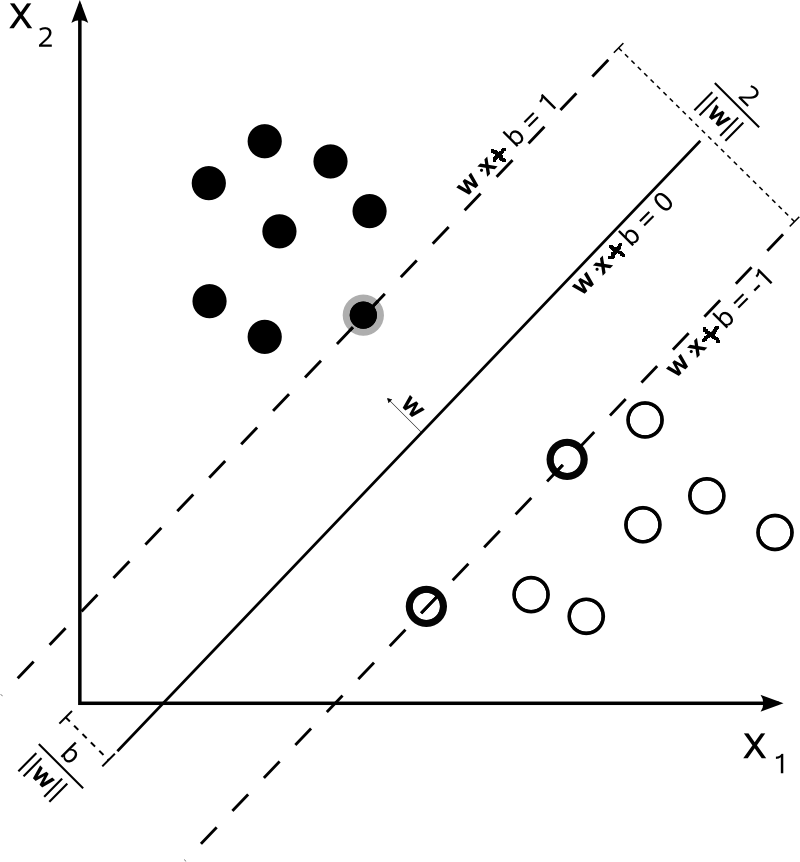
\includegraphics[scale=0.3]{./svm.png}
  \caption{Optimal hyperplane which separates a linearly separable dataset}
  \end{figure}

  \noindent This optimization is generally solved by introducing the Lagrangian:
  \begin{equation}
  L(w,b,\alpha) = \frac{1}{2} \norm{w}^2 - \sum_{i = 1}^{N} \alpha_i [ y_i ( w^T x_i + b) - 1 ]
  \end{equation} 
  where $\alpha_i$ are dual variables. After substituting stationary conditions, the Lagrangian gives the dual cost function:
  
  \begin{equation}
  W(\alpha) = \sum_i \alpha_i - \frac{1}{2} \sum_{i,j} y_i y_j \alpha_i \alpha_j x_i^{T} x_j
  \end{equation}

  \noindent The optimization is now:
  \begin{eqnarray}
  & \hat{\alpha} = \argmax{\alpha} W(\alpha) \nonumber\\
  & \text{subject to} \quad \alpha_i \ge 0  \quad \text{and} \quad \sum_{i=1}^{N} \alpha_i y_i = 0
  \end{eqnarray}

  \noindent So far, the problem of finding s saddle point for $L(w, b)$ becomes an easier one of maximizing $W(\alpha)$. Once this optimization problem is solved, the decision function to predict new data points is shown as follows:

  \begin{equation}
  f(x) = \text{sign}\bigg(\sum_i y_i \alpha_i x_i^T x + b\bigg)
  \end{equation}
  Please note that in equation (7), the point set $\{x_i\}$ includes all calculated support vectors. Moreover, the training data appears as dot products $x_i^T x_j$ in $W(\alpha)$, and it means that classification could be done in higher or even infinite dimensional space by changing $x_i^T x_j$ into other forms of kernel function. Suppose there is a kernel function $K(x, y)$, the original optimization problem is converted by replacing $x_i^T x_j$ with $K(x_i, x_j)$:

  \begin{equation}
  W(\alpha) = \sum_i \alpha_i - \frac{1}{2} \sum_{i,j} y_i y_j \alpha_i \alpha_j K(x_i, x_j)
  \end{equation}

  \noindent Because this transformation has nothing to do with $\alpha_i$ and $y_i$, the optimization remains the same:
  \begin{eqnarray}
  & \hat{\alpha} = \argmax{\alpha} W(\alpha) \nonumber\\
  & \text{subject to} \quad \alpha_i \ge 0  \quad \text{and} \quad \sum_{i=1}^{N} \alpha_i y_i = 0
  \end{eqnarray}
  Finally, the decision function becomes:

  \begin{equation}
  f(x) = \text{sign}\bigg(\sum_i y_i \alpha_i K(x_i,x) + b\bigg)
  \end{equation}
  As shown above, thanks to the kernel function $K(x_i, x_j)$, nonlinear classification is achieved without projecting data points into higher dimensional space. This clever trick refers to ``kernel trick''. Detailed information can be found at \cite{burges1998tutorial}. \\

  \noindent There are many kernels designed over years, and different kernels have different impacts on recognition performances. In experiments of image recognition, the below four kernel functions have been implemented.
  
    \begin{table}[!ht]
        \begin{center}
        \scalebox{1}{
          \begin{tabular}{cc}
          \hline
          \head{Kernel type} & \head{Kernel function}\\
          \hline
          Linear & $x_i^T x_j$ \\
          Polynomial & $(\gamma x_i^T x_j + r)^d$ \\ 
          RBF & $\exp(-\gamma \norm{x_i - x_j}^2)$ \\ 
          Sigmoid & $\tanh(\gamma x_i^T x_j + r)$ \\ 
          Histogram intersection \cite{barla2003histogram} &  $\sum_{p = 1}^{D} min(x_i^p, x_j^p)$ \\
          \hline
          \end{tabular}
        }
        \end{center}
        \caption{Kernel functions}
    \end{table}

  \noindent Although the above mathematical description of support vector machine seems to be complex, there are lots of open source libraries of SVM. One famous and popular package is LIBSVM \cite{CC01a}. What's better is that sklearn \cite{scikit-learn} provides well defined python wrapper to invoke LIBSVM. All the work facilitates the use of SVM, and it demonstrates the collaboration among researchers all around the world.

\subsection{Earth Mover's Distance (EMD)}
In this subsection, Earth mover' distance will be introduced, and the reason is because later on in video recognition, this kind of distance calculation is going to be heavily used. The rest of this section is organized as follows. Firstly, the mathematical model of earth mover proposed by Rubner, Tomasi and Guibas \cite{rubner2000earth} is presented followed by an example of calculating earth mover distance between two images. Last but not least, experiments have been done to show the effectiveness of EMD, and the result is recorded in the section of experiments.\\

\noindent The earth mover's distance is formulated as the following linear programming problem: Let $P = \{(p_1, w_{p_1} ), . . . , (p_m , w_{p_m} )\}$ be the first signature with $m$ clusters, where $p_i$ is the cluster representative and $w_{pi}$ is the weight of the cluster; $Q=\{(q_1,w_{q_1}),...,(q_n,w_{q_n})\}$ the second signature with $n$ clusters; and $D = [d_{ij}]$ the ground distance matrix where $d_{ij}$ is the ground distance between clusters $p_i$ and $q_j$. We want to find a flow $F = [f_{ij}]$, with $f_{ij}$ being the flow between $p_i$ and $q_j$, that minimizes the overall cost: 
\begin{eqnarray}
\text{minimize} & Work(P , Q, F) = \sum_{i=1}^{m}\sum_{j=1}^{n}d_{ij}f_{ij} \nonumber\\
\text{subjective to } & f_{ij} \geq 0 \quad \quad 1 \leq i \leq m,  1 \leq j \leq n \nonumber\\ 
& \sum_{j=1}^n f_{ij} \leq w_{p_i} \quad 1 \leq i \leq m \nonumber\\
& \sum_{i=1}^m f_{ij} \leq w_{q_j} \quad 1 \leq j \leq n \nonumber\\
& \sum_{i=1}^{m} \sum_{j=1}^n f_{ij} = min(\sum_{i=1}^m w_{p_i}, \sum_{j=1}^n w_{q_j}) 
\end{eqnarray}

\noindent Once the above linear programming problem is solved, the earth mover's distance is defined as the resulting work normalized by the total flow:
\begin{equation}
EMD(P, Q) = \frac{\sum_{i=1}^m \sum_{j=1}^n d_{ij} f_{ij}}{\sum_{i=1}^m\sum_{j=1}^n f_{ij}}
\end{equation}

\begin{figure}[!ht]
\centering
	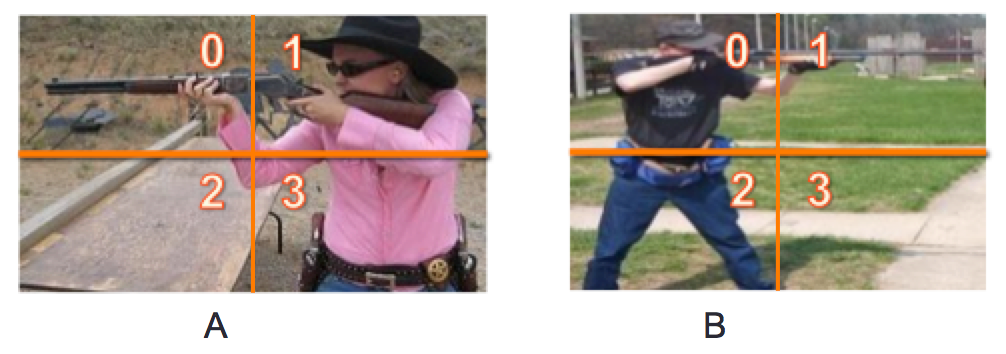
\includegraphics[width=1\textwidth]{./image_EMD_Sample.png}
\caption{Image $A$ and $B$ are divided into 4 parts equally. Then each part is converted into a histogram. Thus, four histograms are stacked to represent each image.}
\end{figure}

\noindent To better understand EMD, here is an example to incorporate EMD into the distance calculation of images. To do so, the first step is to divide each image into four parts equally. An example is depicted in Figure 5. There are two images $A$ and $B$, and they are both divided into 4 parts equally. Each part is then represented by a histogram based on previous built vocabulary. It is easy to see that this division is identical to level 1 in spatial pyramid matching, which also divides an image into 4 equal parts. Now image $A$ and $B$ are represented by 4 histograms each. After adding equal signature value to these histograms, $A$ and $B$ are represented as follows:
	$$A = \{(a_0, 0.25), (a_1, 0.25), (a_2, 0.25), (a_3, 0.25)\}$$
	$$B = \{(b_0, 0.25), (b_1, 0.25), (b_2, 0.25), (b_3, 0.25)\}$$
where $a_0, a_1, a_2, a_3$ and $b_0, b_1, b_2, b_3$ are histograms generated from respective parts.\\

\noindent The next steps is to calculate the distance matrix $D$ with each cell $d_{ij}$ representing the distance between $a_i$ and $b_j$. In this case, Euclidean distance is adopted, and the calculated distance matrix is shown below in Table 2.

\begin{table}[!ht]
    \begin{center}
    \scalebox{0.8}{
      \begin{tabular}{ccccc}
      \hline
      \head{} & \head{$b_0$} & \head{$b_1$} & \head{$b_2$} &\head{$b_3$} \\
      \hline
      $a_0$ & 27.06473721	& 23.37733946	& 29.18047292 &	32.61901286\\
    	$a_1$ & 20.84466359	& 21.50581317	& 21.70253441 &	30.34798181\\
    	$a_2$ & 26.48584528	& 27.38612788	& 27.46816339 &	34.71310992\\
    	$a_3$ & 19.31320792	& 24.20743687	& 21.59861107 &	31.81194744\\
      \hline
      \end{tabular}
    }
    \end{center}
    \caption{Distance matrix between image $A$ and $B$}
\end{table}

\noindent If EMD is not used meaning that there is no alignment of image segments, $a_0$ is matched to $b_0$, $a_1$ is matched to $b_1$, $a_2$ is matched to $b_2$ and $a_3$ is matched to $b_3$. As a result, distance without alignment is calculated as below: $$distance_{unaligned} = d_{00} + d_{11} + d_{22} + d_{33} = 107.851$$

\noindent However, if EMD is used, the best matches between image segments will be found after the linear programming problem in EMD is solved. For image $A$ and $B$, the best matches found are shown in Figure 6. Compared with unaligned case, this one matches the gun and human body properly. Following the matches in Figure 6, distance with alignment is calculated as below: $$distance_{aligned} = d_{30} + d_{12} + d_{01} + d_{23} = 99.106$$

\begin{figure}[!ht]
\centering
	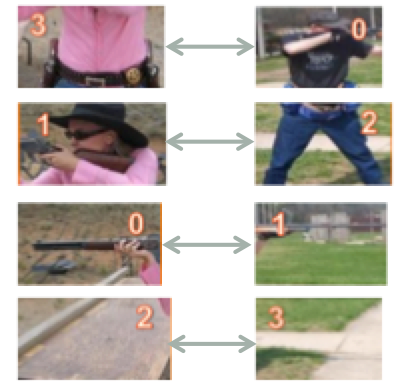
\includegraphics[scale = 1]{./image_EMD.png}
\caption{Matches between segments of $A$ and $B$ calculated by EMD. As we can see, the gun, human body and ground are matched properly. Therefore, distance with alignment shall be more accurate.}
\end{figure}

\noindent Now that the calculation of distances between images  has been defined, it is needed to select a kernel type for SVM to recognize. Apart from RBF (also called as Gaussian kernel) introduced before, three more kernel types were tried in experiments, and they are listed in Table 3. Details of performances of these four kernel types are presented in the experiment section. 
\begin{table}[!ht]
    \begin{center}
      \begin{tabular}{cc}
      \hline
      \head{Kernel type} & \head{Kernel function}\\
      \hline
      Gaussian & $\exp(-\gamma D^2(I_i, I_j)$ \\
      Laplacian & $\exp(- \sqrt{\gamma} D(I_i, I_j)$ \\
      ISD & $\frac{1}{\gamma D^2(I_i, I_j) + 1}$ \\
      ID & $\frac{1}{\sqrt{\gamma}D(I_i, I_j) + 1}$\\
      \hline
      \end{tabular}
    \end{center}
    \caption{Four kernel types which have been tested. $D(I_i, I_j)$ represents the distance between $I_i$ and $I_j$. The kernel parameter $\gamma$ is selected to be the default one $\gamma = \frac{1}{A}$, where $A$ is the mean value of the squared distances between training samples as suggested in \cite{laptev2008learning}.} 
\end{table}

\subsection {Key Frame Identification in a Cluster of Images}
A video could be simplified as a cluster of consecutive frames. By noticing that some consecutive frames in video are similar to each other, it is thought that video can be described by several key frames. In doing so, the data to represent each video can thus be largely reduced. One key step in key frame identification is to check whether two images are near duplicate. If two or more images are examined to be near duplicate to each other, only one image will be selected to represent these images. The rest of this section will focus on two parts: near duplicate identification and how to apply near duplicate identification into key frame identification in videos.

\subsubsection{Identifying near duplicate}
The way which has been implemented to check whether two images are near duplicate follows the method stated on paper \cite{zhao2007near}. In this paper, there are basically three steps to check whether two images are near duplicates. Firstly, the authors propose to use a hash table to match SIFT points. Secondly, a SVM classifier is built based on the matching SIFT points. Finally, this classifier could be used to check near duplicates. Due to a lack of training set, the classifier is not built and thus has to be replaced by threshold checking. In other words, two images are treated as near duplicates as long as the number of matching interest point is large enough compared with a predefined threshold. \\

\noindent In order to minimize false matches, the authors propose one-to-one symmetric matching \cite{zhao2007near}, which ensures all the matches are nearest neighbors. One the other hand, the symmetric property makes sure that the matching result of set A to B is exactly the same as B to A. Suppose there are two images $I_1$ and $I_2$, the steps to check whether these two images are near duplicate go as below:

\begin{enumerate}
  \item{\bfseries Perform PCA on SIFT features of $I_1$ and $I_2$ to reduce dimensions}
  The dimension of SIFT feature is reduced from 128 to 36, and each value of reduced feature is normalized to be within the range [0, 2]. 

  \item{\bfseries Hash all interest points of $I_1$ into a $8 \times 36$ table}

  \begin{figure}[!ht]
  \centering
    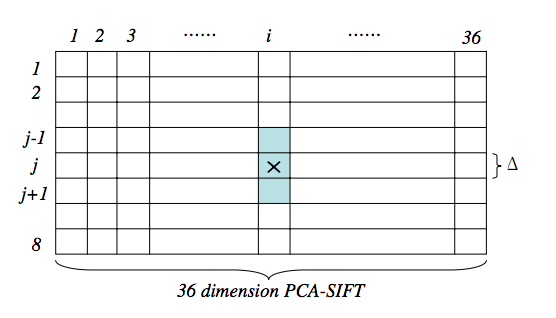
\includegraphics[scale = 0.8]{./hashTable.png}
  \caption{$8 \times 36$ Hash Table \cite{zhao2007near}}
  \end{figure}
  
  The hash table is composed of $8 \times 36$ bins as shown in Figure 7. Given each point $P = [p_1, p_2,..., p_{36}]$ of $I_1$, the index of $p_i$ is hashed to, 
  $$H(p_i) = \lfloor p_i \times 4 \rfloor$$ 
  Since the dimension is 36, $P$ is repeatedly indexed into the corresponding bin for 36 times, according to its quantized value in a particular dimension.   
  
  \item{\bfseries For each interest point $Q$ of $I_2$, examine whether there is a match in $I_1$}\\
  There are three sub steps to go:
    
    \begin{enumerate}
    \item {Hash $Q$ into the hash table}
    \item {Retrieve the set $A(Q)$ satisfying the below constraints}\\
    For each interest point $P \in I_1$, put $P$ into $A(Q)$ if $$\sum_{i=1}^{36}f(q_i, p_i) = 36$$ 

    where 
    \begin{equation*}
        f(q_i, p_i) = \begin{cases}
                   1     & \text{if } \left|H(q_i) - H(p_i)\right| \leq 1\\
                   0 & \text{otherwise}
               \end{cases}
    \end{equation*}

    \item {If $A(Q)$ is not empty, find the nearest neighbor $M \in A(Q)$ with one-to-one symmetric constraint as $Q$' match}
    \end{enumerate}

  \item{\bfseries If the number of matching interest point is large enough, $I_1$ and $I_2$ are near duplicates}
\end{enumerate}

\noindent An example of performing the above algorithm is depicted below in Figure 8. Those colored lines in the upper two images connect the matched interest points, and it is easy to distinguish that the matching accuracy is quite high because of one-to-one constraint \cite{zhao2007near}. Please also notice that only partial matching points are drawn for better visualization. 
  \begin{figure}[!ht]
  \centering
    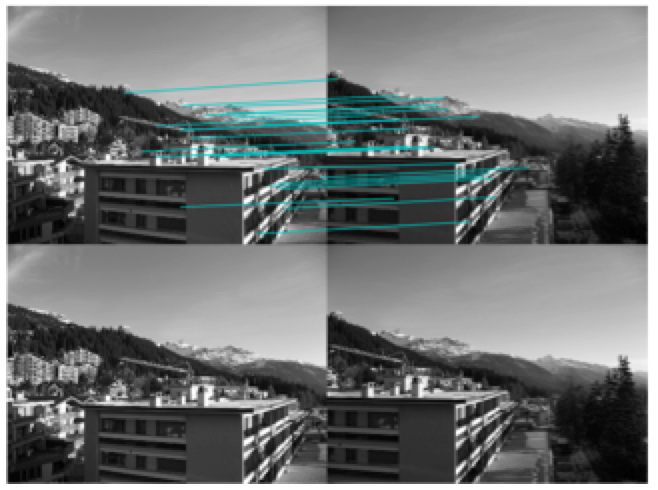
\includegraphics[]{./match.png}
  \caption{Near duplicate example. The colored lines in upper two images connect partial matched interest points, and the below two images are original images.}
  \end{figure}

\subsubsection{Identifying key frames} 
Now that near duplicate method is introduced, it is time to check how this method could be incorporated into key frame identification. The naive brute-force identification checks any two frames in a video, and the computational cost is $O(cn^2)$, where $c$ is the cost of identification and $n$ is the number of all frames. Because $c$ is almost fixed, the left way to reduce computational time is to reduce $n$. Inspired by the paper \cite{wang2012event}, it is recommended to perform K-means algorithm on all the frames at first. Later on, the previous introduced near duplicate identification is performed within each cluster. In this case, if all clusters have equal size, the cost becomes $O(cn^2/r)$, where $r$ is the number of clusters.\\

\noindent Once the clusters are calculated through K-means, the steps to identify key frames in each cluster go as below:

\begin{enumerate}
  \item{\bfseries Build a graph for each cluster}\\
  Each image in that cluster is treated as a node. If two images are identified as near duplicates, an edge is established between these two image nodes. Once all combinations are processed, a graph is built.

  \item{\bfseries Choose representative nodes from the graph}\\
  The first thing to do is to check whether there are connected components in the graph. For each connected component, the node with the largest number of edge is selected to be a key frame. If there is a tie, the key frame is then randomly chosen among candidates. \\

  A very good example is illustrated in Figure 9. These frames are sampled at a rate of one frame per second from a video introducing how to use Google glass from Youtube. Figure 9 depicts how a cluster is processed to produce key frames. There are three connected components inside this cluster. Next, one key frame is extracted from each connected component, and all the three resulting frames are treated as three key frames of this cluster. Because all similar frames are discarded, these three resulting frames are indeed representative. 
\end{enumerate}

  \begin{figure}[!ht]
  \centering
    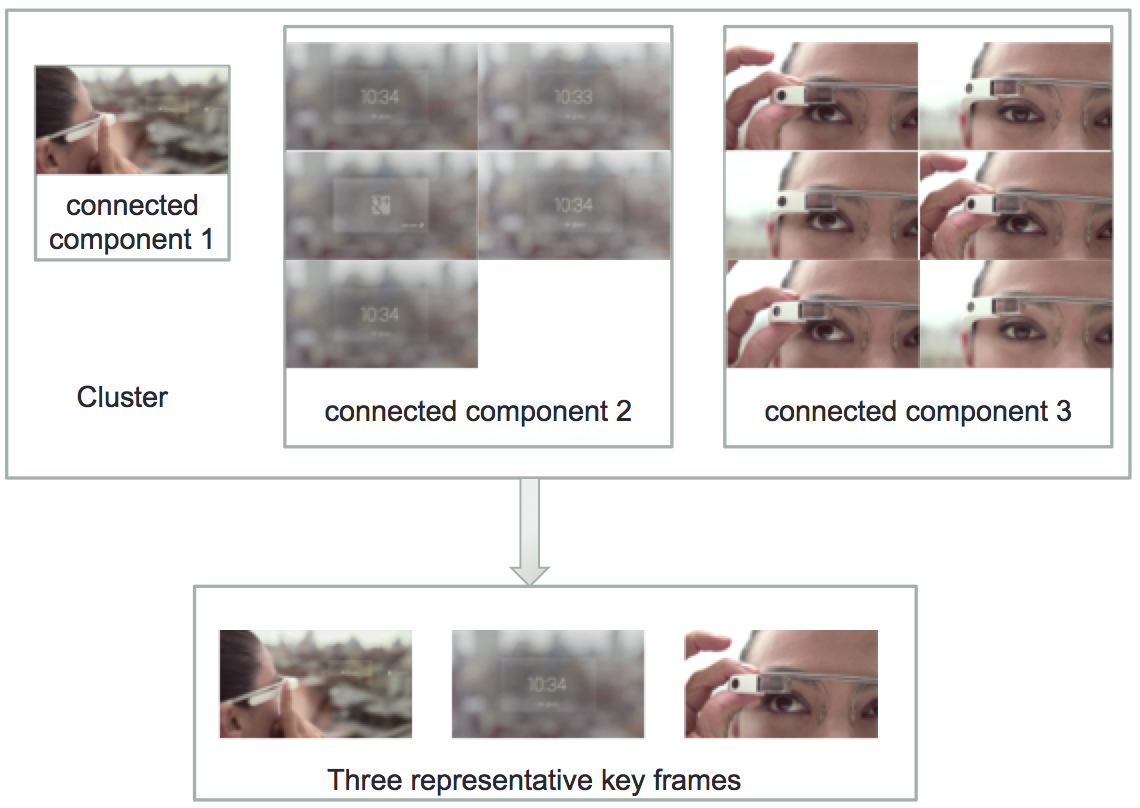
\includegraphics[scale = 0.6]{./keyFrames.png}
  \caption{Key frames identification example. In this cluster, there are three connected components. One frame is selected from each connected component. The resulting three frames are treated as representative frames.}
  \end{figure}

\noindent By combining all representative frames from all clusters, a video could be represented by those key frames. Therefore, the size of video is decreased to some degree and thus accelerates the process of recognition. 



\section {Video Recognition}
As introduced in the section of image recognition, recognition tasks could be simplified into a problem of calculating distances between different samples in the evaluated data set. This is because once the distance matrix is calculated, this distance matrix could be input into K-nearest neighbor algorithms or better approaches like Support Vector Machine for recognition. However, it is not so easy to compare two raw videos in quantitative way and thus difficult to calculate distances using raw video data. In order to resolve this problem, a compact representation similar to image for each video clip is needed. \\

\noindent The rest of this section is organized as follows. Firstly, two different representations of video are introduced followed by the distance calculation for each of these two representations. Once the task of calculating distances is finished, four types of kernels used in image recognition are tested. Finally, another method using concept attributes is presented. 

\subsection{Representations of Videos}
	\subsubsection{Bag of words (BoW)}
	\paragraph{Naive BoW}
	Video consists of a series of consecutive frames and generally presents frames at rates ranging from 20 to 50 frames per second. To be simple, frames sampled from a video every one second could be used to represent this video. For instance, a two-minute video is then represented by 120 frames. With the same representation of image illustrated in section of image recognition, these 120 frames are then converted into 120 histograms. At last, these 120 histograms are stacked to represent this two-minute video. \\

	\noindent A formal description of this approach to build bag of words model for videos go as below.
	\begin{enumerate}
		\item{\bfseries Build vocabulary}\\
	    Similar to image recognition, a vocabulary is needed to represent each frame of videos as a histogram. The vocabulary is built by applying Mini-Batch K-Means \cite{sculley2010web} clustering algorithm on SIFT features of sampled frames for all available videos. In the experiments, two vocabularies were built with the numbers of centroids being 2500 and 1000.

	    \item{\bfseries Represent each video as a stack of histograms}\\
	    Let's say the number of sampled frame in a video is $M$, and each video is represented as a $1 \times V$ histogram, where $V$ is the size of vocabulary. Then histograms of these frames from this video are stacked together to form a $M \times V$ matrix, and this matrix represents this video. 
	\end{enumerate}

	\noindent Following the above steps, videos are converted into a compact matrix with each row representing a frame. However, different videos are converted into matrices with different rows because of different durations. Such differences make it not easy to use general distance calculation formula to calculate video-to-video distance. The solution to this problem will be presented in next section about distance calculation.

	\paragraph{Better BoW}
	In naive Bow, SIFT feature are assigned to its nearest word, and the respective bin in histogram is increased by one. Two questions arise from this statement. Why SIFT feature can only be assigned to one word but not multiple words? Why the respective bin is increased by one but not some other values? To answer these two problems, soft assignment and different weighting schemes are introduced. 

	\begin{itemize}
		\item{Soft assignments}\\
		Soft assignment allows that a visual feature could be assigned to multiple words rather than only one word. In doing so, more valuable information is retained during quantization process and thus might provide more discriminative power. A straightforward approach \cite{jiang2007towards} is that the top N nearest words are selected for each visual feature. Let's say the size of vocabulary is $K$, and thus a $K$-dimensional vector $T = [t_1, t_2,..., t_K]$  is used to represent an image. The algorithm to construct this vector goes as below.\\

		  \begin{algorithm}
		  \caption{Build histogram with soft assignment}
		  \begin{algorithmic}[1]
		  \State Given: vocabulary size $K$, words in vocabulary $[w_1, w2,..., w_k]$, visual features $F$, parameter $N$
		  \State Initialize a $K$-dimensional vector $T = [t_1, t_2,..., t_K]$ with all components $t_i = 0$ 
		  \State
		  \For {$f \in F$ }
		  \State Retrieve the top $N$ nearest words to $f$
		  \State Put the indexes of the top N words in $W_N$ in sorted distances order
			  \State $v \gets 0$
			  \For {$index \in W_N$}
			  	\State $t_{index} \gets t_{index} + \frac{1}{2^v}$
			  	\State $v \gets v + 1$
			  \EndFor
		  \EndFor
		  \State
		  \State return $T$
		  \end{algorithmic}
		  \end{algorithm}

		 The above algorithm selects the top $N$ nearest neighbors. What if $N$ equals to the size of vocabulary? Here, instead of the original algorithm, Agaral and Triggs \cite{agarwal2006hyperfeatures} proposed to use Gaussian mixture model (GMM) built from training data to perform assignment. Let's say the number of components in Gaussian mixture model is $K$. For each visual feature, GMM produces a $K$-dimensional vector representing posterior mixture-component membership probabilities. Finally, all these $K$-dimensional vectors are summed up to produce one final $K$-dimensional vector to represent the respective image. 

		\item{Weighting schemes}\\
		In previous implementation of constructing histograms, only term (word) frequency is taken into consideration. Such implementation ignores global information because the frequencies of words in the global corpus are not considered at all. To address this problem, {\em inverse document frequency(idf)} has already been proposed in information retrieval and becomes rather important \cite{salton1988term}. {\em Inverse document frequency} of visual word $t_i$ is defined as follows. 
		\begin{equation}
		idf(t_i) = \log(N / n_i)
		\end{equation}
		where $N$ is the total number of images in the corpus, and $n_i$ is the number of images having visual word $t_i$. According to this formula, the more frequent a visual word is, the smaller $idf$ is. Therefore, if $tf_i \cdot idf_i$ is used to replace $tf_i$, the weights of words which occur frequently are diminished while the weights of words which occur rarely are increased. Another factor is whether to normalize the vector or not. By taking all these factors into consideration, different weighting schemes are summarized in the below Table 4. Experimental results of these weighting schemes are demonstrated in the section of experiments.

		\begin{table}[!ht]
        \begin{center}

          \begin{tabular}{ccc}
          \hline
          \head{Name} & \head{Factors} & \head{Value for $t_i$}\\
          \hline
    		bxx & $binary$ & 1 if $t_i$ presents, 0 if not \\
    		txx & $tf$ & $tf_i$ \\
    		txc & $tf, normalization$ & $\frac{tf_i}{\sum_i tf_i}$ \\
    		tfx & $tf, idf$ & $tf_i \cdot \log(\sfrac{N}{n_i})$ \\
    		tfc & $tf, idf, normalization$ & $ \frac{tf_i \cdot \log(\sfrac{N}{n_i})}{\sum_i tf_i \cdot \log(\sfrac{N}{n_i})}$ \\
          \hline
          \end{tabular}

        \end{center}
        \caption{Weighting schemes for visual-word feature \cite{yang2007evaluating}. Note that $tf_i$ is number of times a visual word $t_i$ appears in an image, $N$ is the total number of images in the corpus, and $n_i$ is the number of images having visual word $t_i$.}
    	\end{table}
	\end{itemize}

	\subsubsection{Gaussian mixture models}
	In the previous section which talks about employing bag of word model to represent videos, one approach to perform soft assignment is achieved through Gaussian mixture models (GMM). Actually, there are more things that GMM could do. Zhou et al. \cite{zhou2008sift} proposed to represent videos as specialized GMM, which is originally used in speaker verification \cite{reynolds2000speaker}. Because generally the number of features for only one is not enough to robustly learn the parameters of specialized GMM, in order to better build a specialized GMM for each video, there are two steps. The first step is to construct a global GMM on all available features. Secondly, specialized GMMs are derived from the global GMM in an Maximum a Posteriori way. Details of these two steps are presented as follows.

	\begin{figure}[!ht]
	\centering
		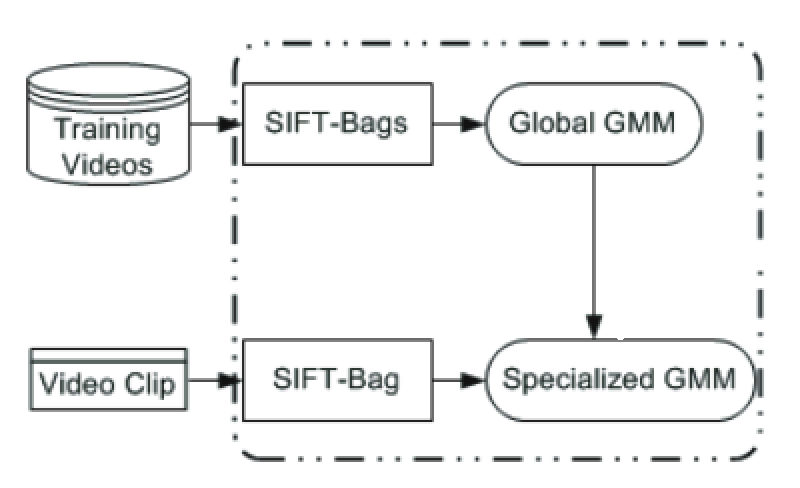
\includegraphics[scale=0.4]{./gmm.png}
	\caption{Illustration of building specialized GMMs for videos \cite{zhou2008sift}. The first step is to build a global GMM based on SIFT features of training data. The second step is to derive a specialized GMM from the global GMM for each video clip.}
	\end{figure}
	\paragraph{Global GMM built from training data} 
	Once all SIFT features of training data are loaded into memory, K-means clustering algorithm is applied on this bag of SIFT features to initialize $K$ centroids, where $K$ is a predefined number determining the number of Gaussian components of the global GMM. Afterward, the standard Expectation-Maximization (EM) is applied to obtain the global GMM. \\

	\noindent Suppose $X = \{x_1, \cdots, x_n\}$ are SIFT features extracted from training data, and $W = \{w_1, \cdots, w_K\}$ are the weights of respective Gaussian component. In E-step, the responsibilities of each SIFT feature to each Gaussian mixture component shall be computed. The below formula depicts the responsibility of $x_i$ to component $k$.
	\begin{equation}
	Pr(k|x_i) = \frac{w_k \cdot \mathcal{N} (x_i ; \mu_k, \Sigma_k) }{\sum_{j=1}^{K}w_j \mathcal{N}(x_i ; \mu_j, \Sigma_j)}
	\end{equation}   

	\noindent In M-step, parameters of each Gaussian component are updated.
	\begin{equation}
	w_k = \frac{\sum_{j=1}^{n} Pr(k|x_j)}{n}
	\end{equation}

	\begin{equation}
	\mu_k = \sum_{j=1}^{n} \big( x_j \cdot \frac{Pr(k|x_j)}{\sum_{l=1}^{K} Pr(l|x_j)} \big)
	\end{equation}

	\begin{equation}
	\Sigma_k = \sum_{j=1}^{n} \big(  (x_j - \mu_k)(x_j - \mu_k)^T \cdot \frac{Pr(k|x_j)}{\sum_{l=1}^{K} Pr(l|x_j)} \big)
	\end{equation}

	\noindent The above E-step and M-step are repeated until convergence, and the resulting distribution of $X$ is modeled by Gaussian mixture models as 
	\begin{equation}
	p(x_i; \Theta) = \sum_{k=1}^{K} w_k \mathcal{N}(x_i; \mu_k, \Sigma_k)
	\end{equation}
	where $\Theta = \{w_1, \mu_1, \Sigma_1, \cdots \}$, $w_k$, $\mu_k$ and $\Sigma_k$ are the weight, mean and covariance matrix of the $k$th Gaussian component. 

	\paragraph{Specialized GMM by adaption}
	The specialized GMM for video clip is built on the global GMM. Given $Z = \{z_1,\cdots,z_H\}$ as the SIFT features extracted from one video clip that is being modeled, a modified EM algorithm is used to calculate the specialized parameters for this video clip. \\

	\noindent In E-step, the posterior probability is calculated as
	\begin{equation}
	Pr(k|z_i) = \frac{w_k \cdot \mathcal{N} (z_i ; \mu_k, \Sigma_k) }{\sum_{j=1}^{K}w_j \mathcal{N}(z_i ; \mu_j, \Sigma_j)}
	\end{equation}   

	\begin{equation}
	n_k = \sum_{i=1}^{H}Pr(k|z_i)
	\end{equation}

	\noindent In M-step, mean vectors are updated as
	\begin{equation}
	E_k(Z) = \frac{1}{n_k} \sum_{i=1}^{H} Pr(k|z_i) z_i
	\end{equation}
	\begin{equation}
	\hat\mu_k = \alpha_k E_k(z) + (1 - \alpha_k) \mu_k
	\end{equation}

	\noindent where $\alpha_k = \sfrac{n_k}{(n_k + r)}$, and $r$ is adjusted empirically depending $H$, the total number of SIFT features for each video clip.\\

	\noindent The E-step and M-step are repeated until convergence. In the end, specialized GMM is modeled as $\hat\theta = \{\hat\mu_1, \cdots, \hat\mu_K \}$. It is worthy noting that all video clips are thus converted into equal size vectors if $\hat\theta$ is treated as a vector.

\subsection{Distance Calculations}
	Now that videos are represented in either stack of histograms or specialized GMM, it is time to calculate video-to-video distance for these two representations. For bag of word model, EMD is incorporated into distance calculation. Given the property that EMD only needs the best matches between segments, the distance between videos with different frames could also be calculated. This idea is originally proposed by Xu and Chang \cite{xu2007visual}, and it is now extended to Aligned Space-Time Pyramid Matching \cite{duan2012visual}. For specialized GMM representation, the author \cite{zhou2008sift} propose a distance formula generated from Kullback-Leibler divergence based on the assumption that the covariance matrices are unchanged during the Maximum a Posteriori adaption process.
	
	\subsubsection{Aligned space-time pyramid matching}
	Let's say there are two videos: $P = \{p_1, \cdots, p_m\}$ and video $Q = \{q_1, \cdots, q_n\}$, where $p_i$ and $q_i$ are the respective histograms in $P$ and $Q$. After attaching equal signatures to $P$ and $Q$ separately based on their number of histograms, $P$ and $Q$ are transformed into
	$$P = \{(p_1, 1 / m),...,(p_m, 1 / m) \}$$
	$$Q = \{(q_1, 1 / n),...,(q_n, 1 / n) \}$$
	
	\noindent Given the above representation, the distance between $P$ and $Q$ are defined as follows:
	\begin{equation}
	D_{PQ} = \frac{\sum_{i=1}^m \sum_{j=1}^n d_{ij} f_{ij}}{\sum_{i=1}^m\sum_{j=1}^n f_{ij}} 
	\end{equation}
	where $[d_{ij}]$ is the ground distance matrix, $d_{ij}$ calculates the distance between $p_i$ and $q_j$, and $[f_{ij}]$ is the optimal flow that can be obtained by solving the below linear programming problem:
	\begin{eqnarray}
	\text{minimize} & \sum_{i=1}^{m}\sum_{j=1}^{n}d_{ij}f_{ij} \nonumber \\
	\text{subjective to} & f_{ij} \geq 0 \quad \quad 1 \leq i \leq m,  1 \leq j \leq n \nonumber \\
	&\sum_{j=1}^n f_{ij} \leq 1 / m \quad 1 \leq i \leq m \nonumber \\
	&\sum_{i=1}^m f_{ij} \leq 1 / n \quad 1 \leq j \leq n\nonumber \\
	&\sum_{i=1}^{m} \sum_{j=1}^n f_{ij} = 1 
	\end{eqnarray}

	\noindent According to \cite{duan2012visual}, the distance calculated through the above process refers to Level-0 distance, and the reason is because a video is treated as a whole rather than several subclips. To utilize the power of pyramid, each video clip is divided into $8^l$ nonoverlapped space-time volumes over multiple levels, $l = 1,\cdots, L-1$, where the volume size is set to be $\sfrac{1}{2^l}$ of the original video in width, height and temporal dimension. Figure 11 below demonstrates how video is divided into 8 sub videos at level one. 

	\begin{figure}[!ht]
	\centering
		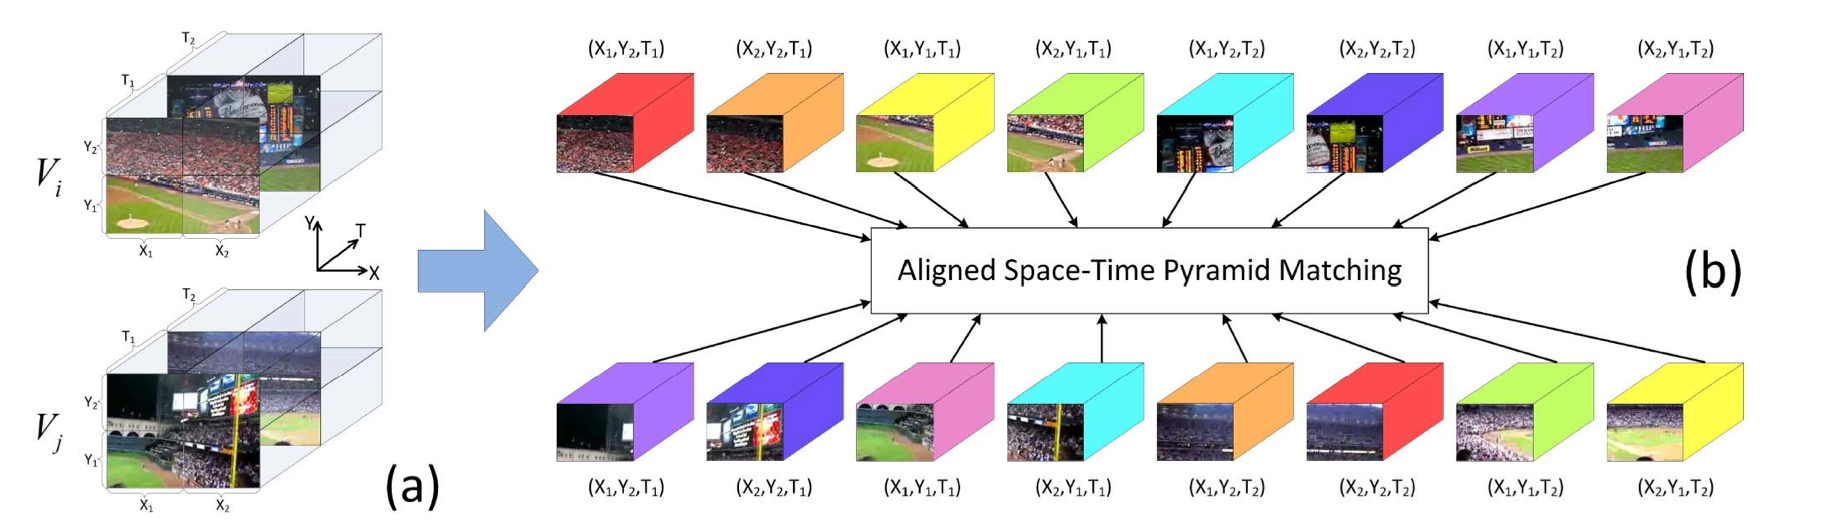
\includegraphics[width=1\linewidth]{./alignedST.png}
	\caption{Illustration of Aligned Space-Time Pyramid Matching at level one \cite{duan2012visual}. (a) Each video clip is divided into 8 sub videos. (b) Matched sub videos are painted in the same color.}
	\end{figure}

	\noindent Compared with level zero distance, the calculation of higher level distances require one more matching stage due to the increasing volumes in videos. Let's say 2 videos $P$ and $Q$ are divided into $8^l$ nonoverlapped space-time volumes at level $l$, and they are represented as
	$$P = (p_1, \cdots, p_R)$$
	$$Q = (q_1, \cdots, q_R)$$
	where $p_i$, $q_j$ are divided space-time volumes and $R$ equals to $8^l$. There are two matching stages to calculate distance between $P$ and $Q$ at level $l$. The first one is to calculate pairwise distance matrix $D$, where $D_{ij}$ is the EMD distance between $p_i$ and $q_j$. As a result, the shape of $D$ is $R^2$ because there are in total $R^2$ matches between space-time volumes of $P$ and $Q$. The additional stage is to align these pairwise distances. After solving the below linear programming problem using integer-flow EMD, those space-time volumes in $P$ and $Q$ are explicitly aligned. 
	\begin{eqnarray}
	& \hat F_{ij} = \argmin{F_{ij}} \sum_{i = 1}^{R} \sum_{j=1}^{R} F_{ij} D_{ij}
	\nonumber \\
	\text{subject to} & \sum_{i=1}^{R} F_{ij} = 1, \quad \forall i \nonumber\\
	&\sum_{j=1}^{R} F_{ij} = 1, \quad \forall j
	\end{eqnarray}

	\noindent Finally, the aligned distance $D_l(P,Q)$ between $P$ and $Q$ at level $l$ can be directly calculated as below
	\begin{equation}
	D_l(P,Q) = \frac{\sum_{i=1}^R \sum_{j=1}^R \hat F_{ij} D_{ij}}{\sum_{i=1}^R \sum_{j=1}^R F_{ij}}
	\end{equation}

	\subsubsection{Distances between specialized GMMs}
	Similar to previous section, let's say there are two video $P$ and $Q$. They are represented as two specialized GMM shown as below.
	$$P = (\mu_1^p, \cdots, \mu_K^p)$$
	$$Q = (\mu_1^q, \cdots, \mu_K^q)$$
	Given global GMM as $\Theta = \{w_1, \mu_1, \Sigma_1, \cdots\}$, the distance of $P$ and $Q$ is
	\begin{equation}
	d(P,Q) = \frac{1}{2} \sum_{k= 1}^{K} w_k (\mu_k^p - \mu_k^q)^T \Sigma_k^{-1} (\mu_k^p - \mu_k^q)
	\end{equation}

\noindent Once video-to-video distances using above approaches are calculated, they will be transformed into Gaussian, Laplacian, ISD and ID kernels for recognition using SVM. Due to the poor performance of KNN, there is no experiment using KNN to recognize videos. 

\subsection{Other Approach: Concept Attributes}
The approaches introduced above are under direct classification category, which model test videos in Bow or GMM and predict their labels directly. However, in real word, many events in videos could be really complex. For example, in the behavior of ``changing a vehicle tire'', events like ``person opening a car'', ``person using wrench'' and ``person holding something'' may be involved. However, Bow and GMM representations fall to catch these low-level events. To be able to better understand complex events, researchers have proposed to use concept attributes to describe images and videos \cite{liu2013video,natsev2010ibm, natarajan2011bbn}. \\

\noindent There are three stages to use concept attributes.
\begin{enumerate}
	\item{\bf Build concept detectors}\\
	Firstly, a concept space $\mathcal{C}^K$, where each dimension encodes the value of a semantic property, is defined. This space is spanned by $K$ concepts $\{C_1, \cdots, C_K\}$. Next, $K$ concept detectors are built based on training data. Each concept detector produces one score of respective concept to each input data sample. 
	\item{\bf Represent data in concept attributes}\\
	Given the above $K$ concept detectors, each data sample is input to these six detectors, and each detector produces one score. As a result, each data sample produces a vector $\{c_1,\cdots, c_k\}$, where $c_i$ is the output score of $i$th concept detector. 
	\item{\bf Recognize event classes using concept attribute representations}\\
	Now videos are transformed into vectors of concept attributes. Such representations are input into classification models like SVM for recognition.
\end{enumerate}

\noindent There are many variations and improvements on the above three stages. For instance, detectors for images could also be used in videos, given that a video consists of multiple frames. If an image is represented as a $K$-dimensional vector, then a video is represented by a $W \times K$ matrix, where each row represents a vector of an image, and there are in total $W$ images. For details, please refer to \cite{liu2013video}. \\

\noindent Last but not least, there are at least two advantages of using concept attributes. The first one is recognizing complex events, which has already been explained. Secondly, pre-trained detectors or even detectors shared by others could also be used to boost recognition performance. Given the fact that the cost of labelling training data is high, the second advantage provides lots of benefits by leveraging available resources. 

% \section{Domain Adaptation}
\subsection{Overview}
So far, all approaches introduced are based on an assumption tha both training data and testing data in recognition come from the same domain, namely, training data and testing data have the same or similar distribution. It works fine if there are enough lablled training data to build up a robust classifier. However, in real world, the most costing and time-consuming process is to label samples and build up training data. At the same time, because of some reasons, there are lots of labelled samples from other domains. For example, here is a task to recognize images from Instagram, and only few images are labelled. With such a small portion of labelled images, it is difficult to build a robust classifier. However, there are thousands of labelled images which could be retrieved through search engines like Google and Bing. Once certain keywords are input to the search engines, lots of relevant images will appear, and the keywords could be used as labels of these retrieved images. Due to the differences in distribution, classifiers built from other domains work poorly in the current domain. But is it possible to utilize these labelled samples from other domains to boost the performance of classifier in the current domain? To address this problem, many domain adaptation methods \cite{daume2007frustratingly, yang2007cross, duan2009domain, duan2012visual}, which utilizes training data from other domains, have been proposed for different proposes, and these methods have been proved to be effective to build robust classifiers with few labelled samples from the target domain. \\


\begin{figure}[!ht]
\centering
  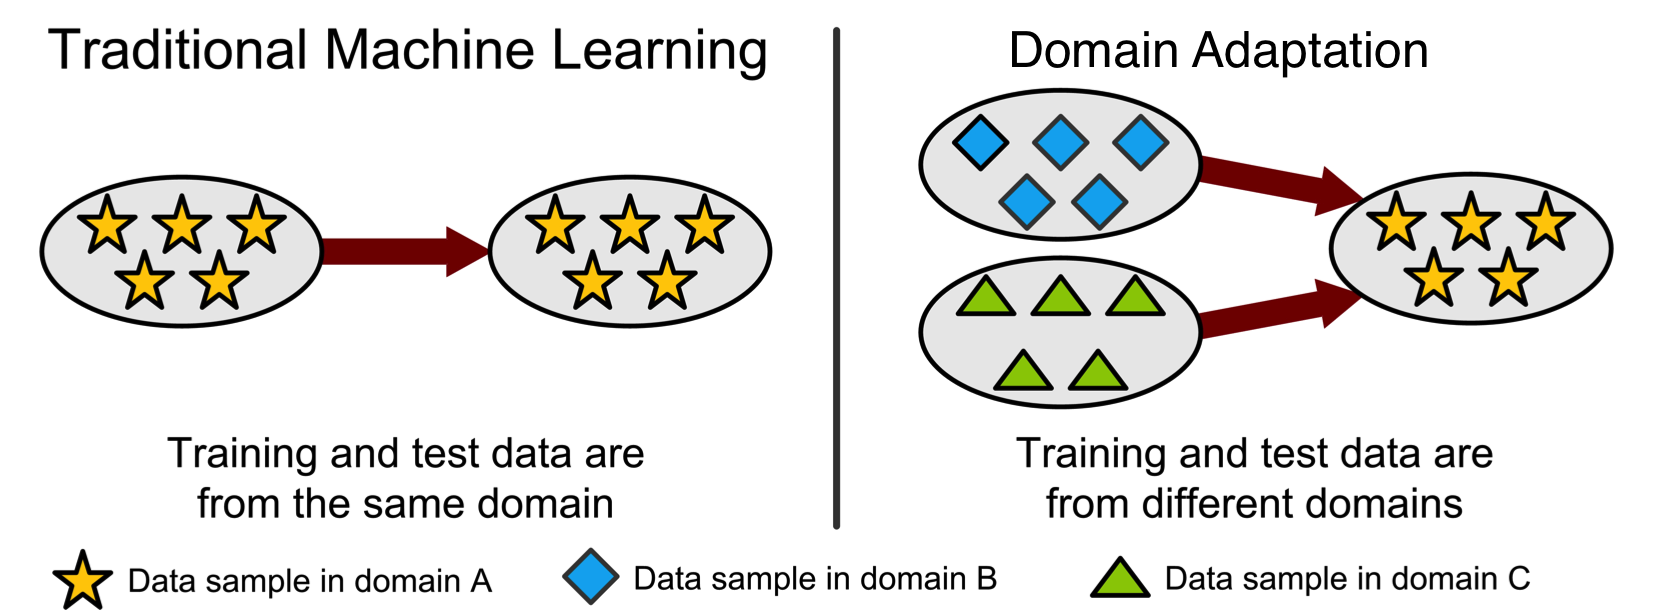
\includegraphics[width=1\textwidth]{./domainAdaption.png}
\caption{Comparison between traditional machine learning and domain adaptation. Data samples from other domains are also used as training data.}
\end{figure}

\noindent As shown in Figure 12, training data and testing data are supposed to come from the same domain in traditional machine learning. In contrast, domain adaptation also utilizes data samples from other domains. Following the terminology from literatures, the target domain, from which the test samples are, is defined as $\mathcal{D}^T$. The other domain, which provides enough labelled data, is defined as auxiliary domain $\mathcal{D}^A$. Moreover, $\mathcal{D}^T = \mathcal{D}_l^T \cup \mathcal{D}_u^T$, where $\mathcal{D}_l^T$ represents limited labelled data, and $\mathcal{D}_u^T$ represents unlabelled data. Also, the auxiliary data set $\mathcal{D}^A = \{(x_i^A, y_i^A)\}_{i=1}^{n_A}$, which is a fully labelled data set. In the rest of this section, domain adaptation methods including Feature Replication \cite{daume2007frustratingly}, Adaptive SVM \cite{yang2007cross}, Domain Transfer SVM \cite{duan2009domain} and Adaptive Multiple Kernel Learning \cite{duan2012visual} are introduced. Experimental results and analysis of these methods are presented in the section of experiments.

\subsection{Feature Replication (FR)}
Feature replication \cite{daume2007frustratingly} uses augmenting features to perform SVM training. There are two different mapping functions to augment samples $\{x\}$ from different domains. 
\begin{equation}
\Phi^T(\mathbf{x}) = (\mathbf{x},\mathbf{x},\mathbf{0}), \quad  \Phi^A(\mathbf{x}) = (\mathbf{x},\mathbf{0}, \mathbf{x})
\end{equation}
where $\Phi^T$ augments samples from $\mathcal{D}^T$, and $\Phi^A$ augments samples from $\mathcal{D}^A$. The kernelized version of the above transformation is pretty straightforward. Suppose the kernel used in SVM projects sample $x$ into higher space through $\theta(x)$. Thus the kernel between $x_i$ and $x_j$ is: $K(x_i, x_j) = \theta(x_i)^T \cdot \theta(x_j)$. After the above augmenting process, 
\begin{eqnarray}
& \Phi_{\theta}^T(x) = (\theta(x), \theta(x), 0) \nonumber \\
& \Phi_{\theta}^A(x) = (\theta(x), 0, \theta(x)) 
\end{eqnarray}
where $\Phi_{\theta}^T(x)$ represents $x$ from $\mathcal{D}^T$ in higher dimensional space, and $\Phi_{\theta}^A(x)$ represents $x$ from $\mathcal{D}^A$ in higher dimensional space. The expanded kernel is defined as $\hat K(x_i, x_j)$. If $x_i$ and $x_j$ come from the same domain, 
\begin{eqnarray}
\hat K(x_i, x_j) &  = & \theta(x_i)^T \cdot \theta(x_j) + \theta(x_i)^T \cdot \theta(x_j) \nonumber \\
 & = & 2 \cdot \theta(x_i)^T \cdot \theta(x_j)   \nonumber \\
 & = & 2 K(x_i, x_j)
\end{eqnarray}
\noindent If  $x_i$ and $x_j$ come from different domains,
\begin{eqnarray}
\hat K(x_i, x_j)  & = &  \theta(x_i)^T \cdot \theta(x_j)  \nonumber \\
 & = &  K(x_i, x_j) 
\end{eqnarray}
\noindent To summarize,  
\[
 \hat K(x_i, x_j) =
  \begin{cases}
   2 K(x_i, x_j) & \text{if } x_i \text{ and } x_j \text{ come from the same domain}\\
   K(x_i, x_j)   & \text{otherwise} 
  \end{cases}
\]
\noindent Based on equations (30) and (31), considering the kernel as a measure of ``similarity'', samples from the same domain are twice as similar as those come from different domains. In order words, for a test sample, those training samples from the same domain  are going to be more influential. Furthermore, the implementation is rather easy since the only operation needed is to twice the kernels of samples from the same domain. 

\subsection{Adaptive Support Vector Machine (A-SVM)}
Adaptive SVM \cite{yang2007cross} incorporates multiple auxiliary classifiers $f_1^A(x), \cdots, f_M^A(x)$ built from $\mathcal{D}^A$ into the standard structure of SVM. The decision function of adapted classifier is defined as
\begin{equation}
f(x) = \sum_{k=1}^M t_k f_{k}^A(x) + \Delta f(x)
\end{equation}
where $\Delta f(x) = w^T \phi(x)$ is called as a {\em permutation function} which is learned from labelled data in the target domain ($\mathcal{D}_l^T$) only, $t_k \in (0, 1)$ is the weight of each auxiliary classifier which sums to one. Because of the change in decision function, the objective function of SVM is changed to be
  \begin{eqnarray}
  & \text{minimize} \quad J(w) = \frac{1}{2} \norm{w}^2 + C \sum_{i=1}^{N}\xi_i  \nonumber \\
  & \text{subject to} \quad \xi_i \ge 0, \quad y_i \sum_{k=1}^M t_k f_{k}^A(x_i) + y_i w^{T} \phi(x_i) \ge 1 - \xi_i \quad \forall i
  \end{eqnarray}
 From the objective function listed above, it is not hard to distinguish that Adaptive SVM aims to find a hyperplane which is not only close to hyperplanes built from $\mathcal{D}^A$ but also separates labelled samples in $\mathcal{D}^T$ well. Due the change of objective function, the Lagrange dual form is changed to be 
  \begin{equation}
  W(\alpha) = \sum_{i} (1 - \lambda_i) \alpha_i - \frac{1}{2} \sum_{i,j} y_i y_j \alpha_i \alpha_j K(x_i, x_j)
  \end{equation}
  where $\lambda_i = y_i \sum_{k=1}^M t_k f_{k}^A(x_i)$. Once the set $\hat \alpha$ which maximizes $W(\alpha)$ is found, the decision function $f(x)$ is expressed as 
 \begin{equation}
f(x) = \sum_{k=1}^M t_k f_{k}^A(x) + \sum_i \hat \alpha_i y_i K(x_i, x)
\end{equation}

\subsection{Domain Transfer Support Vector Machine (DTSVM)}
It has been emphasized that the distributions of $\mathcal{D}^T$ and $\mathcal{D}^A$ are different. Therefore, when these two sets of data are projected into higher dimensional space, their distributions are still distant to each other. If there is a way to reduce the mismatch between $\mathcal{D}^T$ and $\mathcal{D}^A$, then those lablled samples from $\mathcal{D}^A$ could be treated as samples in the target domain to some extent, and of course this is going to improve the performance of recognition because more useful training samples are input to build a robust classifier. Given the fact that fusing multiple kernels helps to increase the performance, Duan et al. \cite{duan2009domain} proposed Domain Transfer SVM (DTSVM) to reduce the mismatch between $\mathcal{D}^T$ and $\mathcal{D}^A$ through calculating the optimal weight of each kernel. Also, the respective classifier is learnt simultaneously. \\

\noindent The mismatch measured by Maximum Mean Discrepancy (MMD) \cite{borgwardt2006integrating} is defined as follows
\begin{equation}
DIST_k(\mathcal{D}^A, \mathcal{D}^T) = \norm{\frac{1}{n_A} \sum_{i=1}^{n_A} \varphi(x_i^A) - \frac{1}{n_T} \sum_{i=1}^{n_T} \varphi{x_i^T}}
\end{equation}
where $x_i^A$ and $x_i^T$ are samples from the auxiliary and target domains, respectively, and $\varphi(x)$ is a mapping function which projects $x$ into higher dimensional space. Given this mapping function, the kernel between $x_i$
 and $x_j$ is $k(x_i, x_j) = \varphi (x_i)^T \cdot \varphi (x_j)$. To simplify equation (36), a column vector $\mathbf{s}$, in which the first $n_A$ entries are $\frac{1}{n_A}$ while the remaining $n_T$ entries are $-\frac{1}{n_T}$. Now the square of MMD in equation (36) is simplified as 
\begin{equation}
DIST_k^2(\mathcal{D}^A, \mathcal{D}^T) = \text{tr}(\mathbf{KS})
\end{equation}
where $\mathbf{S = s s^T }$, and $\mathbf{K = \begin{bmatrix} K^{A,A} & K^{A,T} \\ K^{T, A} & K^{T,T}\\  \end{bmatrix}}$, and $K^{A,A}$, $K^{T,T}$ and $K^{A, T}$ are kernel matrices defined for auxiliary domain, target domain and the cross domain for the auxiliary domain to target domain.\\ 

\noindent According to traditional multiple kernel learning assumption \cite{lanckriet2004learning}, the final kernel $k$ is a result of linear combination of several base kernels $k_1, \cdots, k_M$.
\begin{equation}
k = \sum_{m=1}^{M}d_m k_m
\end{equation}
where $d_m$ is the coefficient of $k_m$ with constraints $d_m \geq 0$ and $\sum_{i=1}^{M}d_m = 1$. Based on final kernel $k$, the decision function is thus defined as
\begin{equation}
f^T(x) = \sum_{m=1}^{M} d_m w_m^T \varphi_m(x) + b 
\end{equation}
where $f^T(x)$ is the permutation function built by $\mathcal{D}_l^T$ based on base kernels with $b$ as the bias term. As a result, once the optimal coefficients $\mathbf{d}=[d_1, \cdots, d_M]^T$ are found through the process of reducing mismatches between $\mathcal{D}^T$ and $\mathcal{D}^A$, this decision function will be easily defined. After incorporating equation (38) into (37), the square of MMD is defined as a function of $\mathbf{d}$.
\begin{equation}
DIST_k^2(\mathcal{D}^A, \mathcal{D}^T) = \Omega(\mathbf{d}) = \mathbf{h^T d}
\end{equation}
where $\mathbf{h} = [tr(\mathbf{K_1 S}), \cdots, tr(\mathbf{K_MS})]^T$, and $\mathbf{K_m} = [\varphi(x)^T \varphi(x)]$ is the $m$th base kernel matrix defined on samples from both auxiliary and target domains. After all these settings, the optimization problem of DTSVM is defined as 
\begin{equation}
\text{minimize} \quad G(\mathbf{d}) = \frac{1}{2} \Omega^2(\mathbf{d}) + \theta J(\mathbf{d})
\end{equation}
where $\theta$ is is a tradeoff parameter which balances the mismatch of distributions and the structural risk function of SVM, and 
  \begin{equation}
  J(\mathbf{d}) = \underset{\boldsymbol{\alpha}}{\max} \; \sum_i \alpha_i - \frac{1}{2} \sum_{i,j} y_i y_j \alpha_i \alpha_j  (\sum_{m=1}^M d_m \; \varphi_m (x_i) ^T \varphi_m (x_j))           
  \end{equation}
To solve the optimization problem, the author \cite{duan2009domain} employed the reduced gradient descent procedure to iteratively update coefficients $\mathbf{d}$ and dual variable $\boldsymbol{\alpha}$. There are two steps:
\begin{enumerate}
	\item{\bf Update the dual variable $\boldsymbol{\alpha}$} \\
	Given the current value $\mathbf{d}$, the optimization problem in equation (42) are  solved by LIBSVM \cite{CC01a}, and the dual variable $\boldsymbol{\alpha}$ is updated.

	\item{\bf Update the linear combination coefficients $\mathbf{d}$}\\
	At $ t+1 $ iteration, $d_{t+1}$ is updated as
	\begin{equation}
	\mathbf{d}_{t+1} = (1 - \eta_t) \mathbf{d}_{t} + \eta_t \mathbf{d}_t^{new}
	\end{equation}
	where $\mathbf{d}_t^{new} = \theta(\mathbf{h h^T} + \varepsilon \mathbf{I_M})^{-1} \mathbf{q}$, and $\varepsilon \mathbf{I_M}$ is added to avoid numerical instability with $\varepsilon = 10^{-5}$, and $\mathbf{q} = [\frac{1}{2}(\boldsymbol{\alpha}_t \diamond \mathbf{y})^T \mathbf{K}_1 (\boldsymbol{\alpha}_t \diamond \mathbf{y}), \cdots, \frac{1}{2}(\boldsymbol{\alpha}_t \diamond \mathbf{y})^T \mathbf{K}_M (\boldsymbol{\alpha}_t \diamond \mathbf{y})]$, and $\eta_t$ is the learning rate. Please note the symbol $\diamond$ represents the element-wise product of two vectors. For formal mathematical induction, please refer to \cite{duan2009domain,duan2012visual} for details, and a formal and concise algorithm description is presented in \cite{duan2012visual}. 
\end{enumerate}

\noindent The above two steps are repeated until convergence or the maximum number of iteration allowed is reached. At the end of this algorithm, the optimal $\mathbf{d}$ is learned as well as the optimal SVM model.

\noindent 
\subsection{Adaptive Multiple Kernel Learning (A-MKL)}
Inspired by adaptive SVM (A-SVM) \cite{yang2007cross} and domain transfer SVM (DTSVM) \cite{duan2009domain}, the authors of DTSVM creatively combined these two approaches and proposed adaptive multiple kernel learning (A-MKL) \cite{duan2012visual}.  A-MKL takes the advantage of pre-learnt classifiers built either from $\mathcal{D}^A$ or $\mathcal{D}^A \cup \mathcal{D}^T$ and defines the decision function as
\begin{equation}
f^T(x) = \sum_{p=1}^{P} \beta_p f_p(x) + \sum_{m=1}^{M} d_m w_m^T \varphi_m(x) + b 
\end{equation}
Compared with equation (39), the added item $\sum_{p=1}^{P} \beta_p f_p(x)$, where $f_1(x), \cdots, f_P(x)$ are pre-learnt classifiers with $\beta$ being the weight of each classifier, represents the influence from pre-learnt classifiers. Because of the influence coming from pre-learnt classifiers, compared with DTSVM, the difference is that equation (42) becomes
\begin{equation}
J(\mathbf{d}) = \underset{\boldsymbol{\alpha}}{\max} \; \sum_i \alpha_i - \frac{1}{2} \sum_{i,j} y_i y_j \alpha_i \alpha_j  (\sum_{m=1}^M d_m \; \breve{\varphi_m} (x_i) ^T \breve{\varphi_m} (x_j))           
\end{equation}
where $\breve{\varphi_m} (x_i) ^T \breve{\varphi_m} (x_j) = \varphi_m (x_i) ^T \varphi_m (x_j) + \frac{1}{\lambda} \boldsymbol{f} (x_i)^T \boldsymbol{f}  (x_j)$, and $\boldsymbol{f}(x)$ is a vector of predictions on $x$ from pre-learnt classifiers $f_1(x), \cdots, f_P(x)$, and $\lambda$ is a regularization parameter in the objective function of SVM. Since the only change is the kernel matrix, once the kernel matrix is fused by scores of pre-learnt classifiers, the algorithm used in DTSVM could be directly employed to calculate the optimal coefficients $\mathbf{d}$ and dual variables $\boldsymbol{\alpha}$. With the help from scores output by pre-learnt classifiers, A-MKL not only reduces the mismatch of distributions between $\mathcal{D}^A$ and $\mathcal{D}^T$ but also finds a hyperplane which is close to the optimal hyperplane of $\mathcal{D}^A$ in ``new'' distribution. 

% \section{Experiments}
\subsection{Image recognition}
\subsubsection{Data set description}
The image data set, in which there are six classes (shooting, playing guitar, running, phoning, riding bike and riding horse) as shown in Figure 13, comes from \cite{li2011actions}. For each class, there are 60 images with different backgrounds, different persons and different viewpoints. 

\begin{figure}[!ht]
\centering
  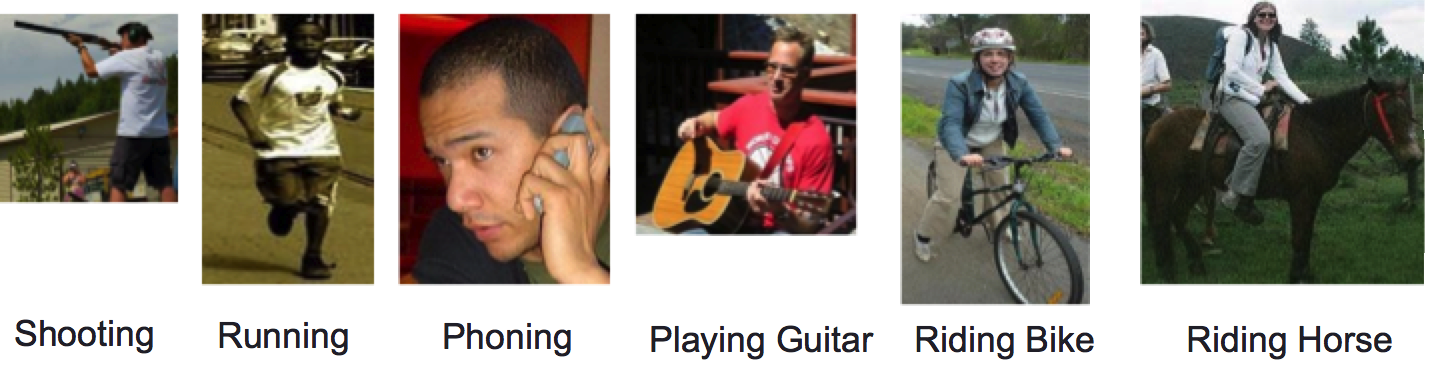
\includegraphics[width=1\textwidth]{./imageSet.png}
\caption{Samples from the image data set used in experiments \cite{li2011actions}}
\end{figure}

\subsubsection{Performance of spatial pyramid matching}
To examine the performance of spatial pyramid matching, a vocabulary with 300 was built from all SIFT features extracted from the total 360 images using Mini-Batch K-Means cluster algorithm. Next, three kinds of pyramids were built: one-level, two-level and three level. In the process of building pyramids, histograms at different levels were concatenated together to form a long vector with respective weights. As a result, one-level pyramid was a 300-dimensional vector, two-level pyramid was a 1500-dimensional vector and three-level pyramid was a 6300-dimensional vector. As for classification, SVM with 5 different kernels and KNN were employed based on different pyramid representations. In this experiment, 40 images each class were randomly chosen to act as training data while the left 20 images each class were used as testing data set. Also, the recognition accuracy is defined as 
\begin{equation}
\text{recognition accuracy} = \frac{\text{correct predictions}}{\text{number of testing samples}}
\end{equation}
where correct predictions represent the number of testing samples which are correctly predicted. The recognition results using the above settings are reported in Table 5 and 6. \\

\begin{table}[!ht]
    \begin{center}

      \begin{tabular} {cccc}
      \hline
    	\head{SVM} & \head{One-level} & \head{Two-level} & \head{Three-level}\\
      \hline
      Linear & 74.17 & 80 & {\bf 87.5} \\
      Poly & 70 & 62.5 & 31.67 \\
      RBF & 37.5 & 83.33 & 74.17 \\
      Sigmoid & 16.67 & 16.67 & 16.67 \\
      Histogram Intersection & 79.17 & 82.5 & {\bf 85} \\
      \hline
      \end{tabular}
    
    \end{center}
    \caption{Recognition accuracies (percent) of different spatial pyramids using SVM with different kernels}
\end{table}

\begin{table}[!ht]
	\begin{center}

	  \begin{tabular} {cccc}
	  \hline
		\head{} & \head{One-level} & \head{Two-level} & \head{Three-level}\\
	  \hline
      KNN & 50.83 & 45 & 48.33 \\
      \hline
      \end{tabular}
    
    \end{center}
    \caption{Recognition accuracies (percent) of different spatial pyramids using KNN}
\end{table}

\noindent Table 5 above reports the recognition accuracies using SVM with different kernels fro different pyramids. The kernel types which projects samples into higher dimensional space like ``Poly'' and ``RBF'' abd ``Sigmoid'' performed much worse than ``Linear'' and ``Histogram Intersection''. Also, it is easy to see that the recognition accuracies increased by fusing information from multiple levels. For ``Linear'' and ``Histogram Intersection'', their performances were improved significantly from one-level pyramid to three-level pyramid, and ``Linear'' achieved the best result $87.5 \%$ while ``Histogram Intersection'' achieved the second best result $85 \%$ at three-level pyramid. Table 6 depicts the performance of KNN when the number of neighbors was set to 5. Compared with reasonable result of SVM, KNN did not perform quite well. The best result achieved at one-level $50.83\%$ is much smaller than $74.17\%$ which was achieved by SVM with ``Linear'' kernel. Such result makes sense because it is generally thought that KNN performs worse than SVM since KNN is a lazy learner which does not consider the global information. 

\subsubsection{Performance of earth mover's distance}
EMD was also experimented to examine its effectiveness in recognition. Following the method introduced before, each image was divided into 4 pieces equally, and EMD attempted to align these 4 pieces. In this experiment, the distance matrix calculated with EMD was referred as aligned distance while the distance matrix without EMD was referred as unaligned distance. Once distances were calculated, they were transformed into four different kernels. Finally, these kernel matrices are input into SVM for classification. Unlike previous division of training and testing samples, this experiment randomly selected $50\%$ images as training data and the other $50\%$ as testing data. The result using the above settings is recorded in Table 7. 

\begin{table}[!ht]
	\begin{center}

	  \begin{tabular} {ccccc}
	  \hline
		\head{} & \head{RBF} & \head{LAP} & \head{ID} & \head{ISD}\\
	  \hline
      Aligned Distance & 79.44 & 76.11 & 73.89 & 75.56 \\
      Unaligned Distance & 78.89 & 75.56 & 73.33 & 75 \\
      \hline
      \end{tabular}
    \end{center}

    \caption{Comparison of recognition accuracy between aligned distance and unaligned distance}
\end{table}

\noindent For all four kernel types, aligned distance performed better than unaligned distance. Though slightly, it shows the robustness of EMD which gives a more accurate image-to-image distance. Also, it is worth noting that these four kernels output different results. So it is important to select a good kernel in order to build a robust classifier. 


\subsection{Video recognition}
\subsubsection{Data set description}
The data set used in this experiment is retrieved from Visual Computing Group of Nanyang Technological University, and this data set has been used for comprehensive experiments in \cite{duan2012visual}. There are two different domains \cite{loui2007kodak}: one comes from the Kodak Consumer Video Benchmark Data set while the other comes from Youtube. Also, there are two types of features: one is SIFT while the other one is space-time feature. According to the accuracies of different feature reported in \cite{duan2012visual}, SIFT is preferred. There are six different classes, and the numbers of videos in each class from different domains are summarized in the below table.

  \begin{table}[!ht]
    \begin{center}
    
      \begin{tabular}{cccccccc}
      \hline
      \head{} & \head{Wedding} & \head{Sports} & \head{Show} & \head{Picnic} & \head{Parade} & \head{Birthday} & \head{Total}\\
      \hline
      Kodak & 27 & 75 & 57 & 6 & 14 & 16 & 195\\
      Youtube & 91 & 260 & 200 & 85 & 119 & 151 & 906\\
      \hline
      \end{tabular}
    
    \end{center}
    \caption{Number of videos in each class from Kodak and Youtube}
  \end{table}

\subsubsection{Performance of aligned space-time pyramid matching}
To examine Aligned Space-Time Pyramid Matching, a visual vocabulary is firstly needed in order to convert videos into stacks of histograms. The visual vocabulary with 2500 words was built on SIFT features sampled from features of Kodak data set. Due to a lack of memory, the size of training data was $167837 \times 128$. Although the training size was relatively small, fortunately, it still produced comparable results compared with performances reported in \cite{duan2012visual}. The next step was to convert all Kodak videos into either one stack of histograms (level 0) or 8 stacks of histograms (level 1) based on the visual vocabulary built before. Once Bow models for all Kodak videos are built, EMD was employed to calculated video-to-video distances among all these videos. In this experiment, the C program wrote by Rubner, who is the proposer of Earth Mover's distance \cite{rubner2000earth}, was used. To integrate this C program with the main codes written in Python, an interface was added to enable communications between these two modules. Please also note that the time taken by calculating level one distances is around 65 times of that taken by calculating level 0 distance. When calculating level one distance, the number of pairwise distances needed is $8 \times 8 = 64$. If the aligned process is also considered, the number of times to invoke EMD becomes 65. However, for level 0 distance, only one time is needed to call EMD when calculating the distance between two videos. Similar to the settings in image recognition, distances were then transformed into kernels using Gaussian, Laplacian, ISD and ID. The final step was to employ SVM to perform recognition based on these gram matrices. Due to the poor performance of KNN, KNN was not tried here. Furthermore, a new mode fusing SVM scores from Gaussian, Laplacian, ISD and ID was tried, and this fusing process is defined as
\begin{equation}
f^{Fuse} = \frac{1}{N} \sum_{i=1}^{N} \frac{1}{1 +\exp{(-f_i)}}
\end{equation}

\noindent where $N$ is the number of classifiers, and $f_i$ is the score output by $i$th classifier. In this case, $N = 4$, and the four SVM classifiers were built from Gaussain, Laplacian, ISD and ID kernel matrices. \\

\begin{table}[!ht]
  \begin{center}
  \scalebox{0.9}{
    \begin{tabular} {cccccc}
    \hline
    \head{} & \head{Gaussian} & \head{Laplacian} & \head{ISD} & \head{ID} &\head{Fused scores}\\
    \hline
    Level 0 & $44.38 \pm 2.13$ & $44.90 \pm 2.73$ & $44.01 \pm 2.13$ & $45.36 \pm 3.13$ & $44.33 \pm 2.61$ \\
    Level 1 (Unaligned) &$43.08 \pm 3.14$ &$43.85\pm3.84$ &$43.22\pm3.11$ &$43.85\pm3.56$ &$43.55\pm3.46$ \\
    Level 1 (Aligned)&$43.61\pm2.97$ &$43.40\pm3.18$ &$43.46\pm2.97$ &$43.22\pm3.11$ & $44.08\pm3.25$ \\
      \hline
      \end{tabular}
      }
    \end{center}
    \caption{Means and standard deviations (percent) of MAPs over six events at different levels using SVM with different kernels.}
\end{table}

\noindent In the experiment shown in Table 9, each time three videos from each class were selected as training data while the rest of Kodak videos were used as testing videos. As a result, 18 videos were used to train models while the rest 177 videos acted as testing videos. Furthermore, SVM was trained in one-against-all manner, which trains in total 6 classifiers for all 6 events. This experiment were repeated for five times, and the mean and standard deviation of Mean Average Precision (MAP) for each method was recorded in Table 9. Given the fact that only around $9.23\% \; (\sfrac{18}{195})$ videos were used as training data, the performance reported in Table 9 was quite good. There are three observations based on results in Table 9. 
\begin{enumerate}
  \item{\bf In this case, Level 0 performs better than both unaligned Level 1 and aligned Lavel 1 for all types of kernel} \\
  The most possible reason is due to a lack of training data. In latter experiments, when all youtube videos and randomly selected 18 Kodak videos were used for training, the performance ranking was: Level 1 (Aligned) $>$ Level 1 (Unaligned) $>$ Level 0. 

  \item{\bf Level 1 (Aligned) performed better than Level 1 (Unaligned) in most cases}\\
  Thus, the one additional alignment makes worthwhile contribution to a better performance though it requires one more call of EMD. 

  \item{\bf the approach of fusing scores provides a guarantee on performance}\\
  For all three cases, the means of MAP using fused scores were always not the worst, and it was even the best for aligned Level 1 distance. Therefore, it provides a good insight that fusing scores of multiple classifiers is a good alternative if the standalone performances of those classifiers are unclear.

\end{enumerate}

\begin{table}[!ht]
  \begin{center}
  \scalebox{0.9}{
    \begin{tabular} {cccccc}
    \hline
    \head{} & \head{Gaussian} & \head{Laplacian} & \head{ISD} & \head{ID} &\head{Fused scores}\\
    \hline
     bxx& $40.20 \pm 2.57$ & $38.35 \pm 2.31$ & $39.93 \pm 2.58$ & $38.23 \pm 2.08$ & $39.34 \pm 2.55$ \\
     txx& $44.28 \pm 2.14$ & $44.90 \pm 2.73$ & $44.01 \pm 2.13 $ & $45.36 \pm 3.13 $ & $44.33 \pm 2.61$ \\
     txc& $ 42.15 \pm 4.73$ & $45.01 \pm 3.45$ & $43.47 \pm 4.56$ & $45.38 \pm 3.20$ & $44.11 \pm 3.90$ \\
     tfx& $ 43.76 \pm 2.99$ & $44.14 \pm 3.36$ & $43.61 \pm 3.03$ & $44.05 \pm 3.51$ & $44.18 \pm 3.22$ \\

     tfc& $ 43.71\pm 1.37$ & $\mathbf{46.02 \pm 1.84}$ & $\mathbf{44.93 \pm 1.64}$ & $\mathbf{46.21 \pm 1.83}$ & $\mathbf{45.28 \pm 1.62}$ \\
     Easy soft& $43.54 \pm 2.12$ & $ 44.77\pm 2.41$ & $43.52 \pm 2.08$ & $45.24 \pm 2.47$ & $ 44.79\pm 2.55$ \\
     Gaussian soft& $\mathbf{44.77 \pm 2.80}$ & $45.23 \pm 2.76$ & $44.90 \pm 3.01$ & $45.23 \pm 2.87$ & $\mathbf{45.20 \pm 3.04}$ \\
      \hline
      \end{tabular}
      }
    \end{center}
    \caption{Means and standard deviations (percent) of MAPs over six events using different mechanisms to build histograms}
\end{table}

\noindent Experiments on building better BoW using different weighting schemes and soft assignment were also tried. Following the same setting of experiments in Table 9, the results of various approaches were recorded in Table 10. ``Easy soft'' represents the approach that the top $T$ neighbors are retrieved for each feature when building histograms. In this experiment, $T = 4$. ``Gaussian soft'' represents the approach which uses Gaussian Mixture Models to build histograms. For other approaches like ``txc'', please refer to Table 4 in the section of representations of videos. Based on results shown in Table 10, it is not easy to that ``tfc'' and ``Gaussian soft assignment'' performs relatively better than the rest approaches. Thus, histograms built through soft assignment and weighting schemes which considers global frequencies of visual words possess more discriminable power. \\

\begin{table}[!ht]
  \begin{center}

    \begin{tabular} {cccc}
    \hline
    \head{Training videos} & \head{Testing videos} &\head{Original videos} &\head{Compressed videos}\\
    \hline
    60 & 846 &  $38.9 \pm 2.9$  & $38.6 \pm 2.8$ \\
    120 & 786 & $45.7 \pm 2.2$  & $44.5 \pm 1.6$ \\
    180 & 726 & $49.5 \pm 1.8$  & $48.3 \pm 1.9$ \\
    240 & 666 & $52.0 \pm 2.1$  & $50.6 \pm 2.1$\\
    \hline
    \end{tabular}

    \end{center}
    \caption{Recognition accuracies (percent) using distances calculated on original Youtube videos and distances calculated on Youtube compressed videos.}
\end{table}
\noindent The approach of identifying key frames in a cluster of images introduced in the section of image recognition was employed to compress Youtube videos. Originally, the total size of Youtube histograms in Python serialization file was 4.42 GB. After compressing, the size was reduced to 3.17 GB, which means around $28.41 \%$ frames were discarded. Then the level 0 distance matrix of compressed Youtube videos using Aligned Space-Time Pyramid Matching was calculated. In this experiment, SVM was trained in one-against-one manner to recognize multiple classes. The distance of original Youtube videos were used as a baseline to compare the performance of compressed videos. Table 11 depicts the recognition accuracies for these two distance matrices using different number of training videos. There are two observations based on Table 11.
\begin{enumerate}
  \item{\bf The performance of compressed videos is slightly worse than original videos} \\
  Though compressed videos contain less redundant frames, the performance is still worse than original videos. The most possible explanation is that EMD always finds the best matches among frames. Thus, those redundant frames are actually ignored during the calculation of distances. As a result, it shows the effectiveness of EMD. 

  \item{\bf With more training samples, the recognition accuracy increases}
  This is actually common sense. With more training samples, the found boundary is more likely to be near to the optimal bounday. However, the problem is there is normally no enough labelled samples. This is also the main reason why researchers are exploring domain adaptations. 
\end{enumerate}

\subsubsection{Performance of specialized GMM}
\begin{table}[!ht]
  \begin{center}
  \scalebox{0.9}{
    \begin{tabular} {cccccc}
    \hline
    \head{} & \head{Gaussian} & \head{Laplacian} & \head{ISD} & \head{ID} &\head{Fused scores}\\
    \hline
    spherical 128& $24.70 \pm 1.41 $ & $ 43.04 \pm 1.61 $ & $26.92 \pm 1.00$ & $\mathbf{43.64 \pm 0.96}$ & $ 32.91 \pm 2.20$ \\
    spherical 64& $ 23.99 \pm 1.40$ & $42.35 \pm 1.64$ & $ 25.62\pm 1.11$ & $43.42 \pm 1.18$ & $29.01 \pm 1.10$ \\
    full 128& $ 25.69 \pm 7.57 $ & $21.39 \pm 7.32$ & $26.49 \pm 8.38$ & $21.93 \pm 7.75$ & $21.79 \pm 7.29$ \\
    full 64& $  25.23 \pm 0.94$ & $ 29.69 \pm 1.81$ & $25.68 \pm 1.34$ & $30.74 \pm 1.67$ & $26.74 \pm 1.63$ \\
    \hline
    \end{tabular}
    }
    \end{center}
    \caption{Means and standard deviations (percent) of MAPs over six events using different GMMs}
\end{table}
\noindent Experiments using another representations of video clips are presented here. There are in total four different settings controlled by the type covariance and the dimension of SIFT feature. Two types of covariances were adopted in experiments: spherical and full. While spherical covariance assumes that the variations on all dimensions are the same, full covariance does not have such assumption. An example to demonstrate the differences of these two types of covariances is Figure 14, where spherical covariance builds Gaussian distributions in circle shape, and full covariance builds in ellipse. Also, the dimension of SIFT was reduced to 64 through PCA for experiments. \\ 

\begin{figure}[!ht]
\centering
  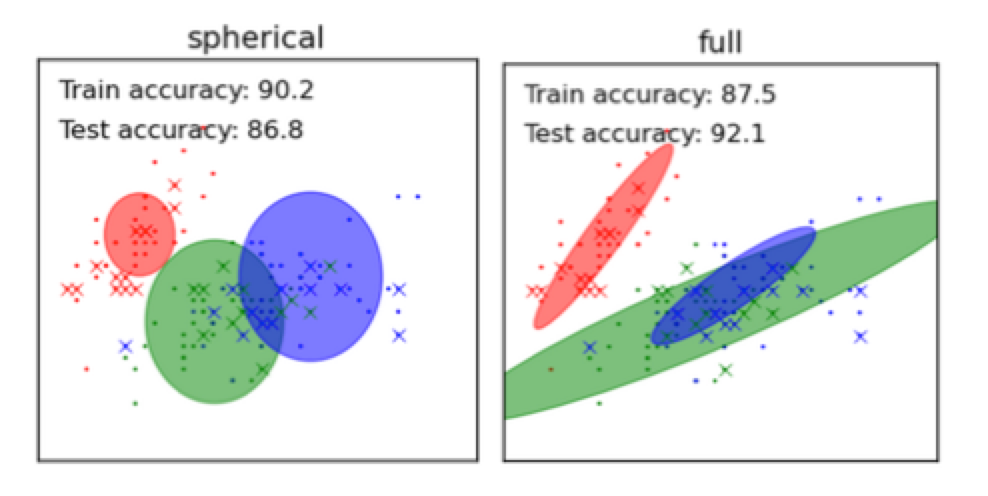
\includegraphics[scale = 0.6]{./DifCov.png}
\caption{Gaussian Mixtures Models built by different covariance types \cite{scikit-learn}.}
\end{figure}

\noindent Based on results in Table 12, there are two observations. 
\begin{enumerate}
  \item{\bf Spherical covariance performed better than full covariance}\\
  Except for Gaussian kernel, the performances of spherical covariance with 128 dimensional SIFT features were better than those of full covariance. The possible reason could be that the number of features was not enough to build good enough specialized GMM for most video clips when full covariance was adopted. 

  \item{\bf Spherical covariance using ID kernel performed the best}\\
  Overall speaking, GMM representations of videos did not perform well compared with Bow representations. However, the best MAP achieved by spherical covariance using 128 dimensional feature reached $43.64 \%$, which is slightly worse than that achieved by level 0 distance using aligned space-time pyramid matching. This gives an insight that a right kernel type helps a lot to improve the performance. 
\end{enumerate}


\subsubsection{Performance of concept attributes}
\begin{table}[!ht]
  \begin{center}

    \begin{tabular} {cc}
    \hline
    \head{} & \head{Recognition accuracy}\\
    \hline
    Kodak $\to$ Kodak & $38.5 \pm 12.7$\\
    Youtube $\to$ Kodak & $30.0 \pm 6.9$\\
    Baseline & $41.6 \pm 11.5$\\
    \hline
    \end{tabular}

    \end{center}
    \caption{Means and standard deviations (percent) of recognition accuracies using concept attributes}
\end{table}
\noindent Concept attribute was also experimented. In this experiment, 2-layer SVM classification structure was implemented, where the first layer built up 6 concept detectors, and the second layer trained and tested videos using 6-dimensional vectors, in which each dimension represented the respective semantic concept like ``birthday'' and ``show''. The results were presented in Table 13. ``Kodak $\to$ Kodak'' represents the case where training samples in Kodak videos were used to train concept detectors, whereas ``Youtbe $\to$ Kodak'' represents the case where all Youtube videos were used to train concept detectors. The second stage SVM was implemented in one-against-one manner with Gaussian kernel. Baseline was implemented using the average kernel generated from 4 types of kernel matrix. Based on results recorded in Table 13, there are two observations.
\begin{enumerate}
  \item{\bf ``Youtbe $\to$ Kodak'' performed much worse than ``Kodak $\to$ Kodak''}\\ This result makes sense since Youtbe videos and Kodak videos come from two different domains. Therefore, their distributions are quite different. 

  \item{\bf ``Kodak $\to$ Kodak'' was slightly worse than baseline}\\
  This observation demonstrates the promising discriminable power of concept attribute. Though the representation of videos is reduced into 6-dimensional vectors, its performance is still comparable with that by basline. Actually, concept attribute could be implemented to perform better by adding more concepts. However, there was no enough training data. 

\end{enumerate}


\subsubsection{Performance of domain adaptation methods}
This subsection introduces the experiments on domain adaptation methods. There are in total four domain adaptations: Feature Replication (FR), Adaptive SVM (A-SVM), Domain Transfer SVM (DTSVM) and Adaptive Multiple Kernel Learning (A-MKL). The other three methods SVM\_T, SVM\_AT and MKL are used as baseline, where SVM\_T only relied on $\mathcal{D}_l^T$, and SVM\_AT relied on training samples from both $\mathcal{D}^T$ and $\mathcal{D}^A$, and MKL used the average of all kernel matrices. Therefore, except SVM\_T, all other 6 methods needed all Youtube videos as training data in $\mathcal{D}^A$. In Table 14, various distance matrices are listed which have been implemented. Once a distance matrix was given, 20 kernel matrices were built, where Gaussian, Laplacian, ISD and ID were employed by setting kernel parameter as $\gamma = 2^l \gamma_0$, and $l \in (-3, -2,\cdots, 1)$. Such setting was made to align with that stated in \cite{duan2012visual}. One special case was MAP(8) in which 2 different distance matrices were input. As a result, there were in total 40 base kernels for MAP(8) during the process of all these methods. As for the division of training samples and testing samples, each time the experiment randomly selected 3 videos from Kodak set as $\mathcal{D}_l^T$ while the left videos were treated as $\mathcal{D}_u^T$. All Youtube videos were used as full labelled set in $\mathcal{D}^A$ if needed. The results of repeating this experiment for five times were recorded in Table 15 as below.\\

\begin{table}[!ht]
  \begin{center}
  \scalebox{0.9}{
    \begin{tabular} {cl}
    \hline
    \head{Setting Name} & \head{Content}\\
    \hline
    MAP(1) & Level 0 distance in aligned space-time pyramid matching \\
    MAP(2) & unaligned Level 1 distance in aligned space-time pyramid matching \\
    MAP(3) & aligned Level 1 distance in aligned space-time pyramid matching \\
    MAP(4) & distances calculated by histograms built in ``tfc'' weighting scheme \\
    MAP(5) & distances calculated by histograms built by straightforward soft assignment \\
    MAP(6) & distances calculated by histograms built by GMM soft assignment \\
    MAP(7) & \vtop{\hbox{\strut distances calculated by specialized GMMs built on 128 dimensional SIFT} \hbox{\strut features with spherical covariance}} \\
    MAP(8) & \vtop{\hbox{\strut two set of distances: aligned Level 1 distances and distances from histograms} \hbox{\strut built through GMM soft assignment}} \\

    \hline
    \end{tabular}
  }
    \end{center}
    \caption{Experimental settings}
\end{table}


\begin{table}[!ht]
  \begin{center}
  \scalebox{0.8}{
    \begin{tabular} {cccccccc}
    \hline
    \head{} &\head{SVM\textunderscore T} &\head{SVM\textunderscore AT} &\head{FR} &\head{A-SVM} &\head{MKL} &\head{DTSVM} &\head{A-MKL} \\
    \hline
    MAP(1) & $44.33 \pm 2.61$ & $52.21 \pm2.54$ & $52.33 \pm 2.20$ & $47.03 \pm3.26$ & $50.82 \pm2.16$ & $47.14 \pm3.26$ & $54.29 \pm 2.21$ \\

    MAP(2) & $43.55 \pm3.46$&  $55.37 \pm2.26$&  $55.95 \pm 3.79$  &$45.86 \pm4.39$ & $55.08 \pm 6.17$  &$50.97 \pm 1.38$ & $54.26 \pm 3.46$ \\
    MAP(3) & $44.08 \pm 3.25$ & $57.56 \pm3.02$ & $53.91 \pm 1.48$ & $45.42 \pm 3.62$ &$53.81 \pm 3.86$ & $53.32 \pm 2.56$ & $\mathbf{57.45 \pm 1.64}$ \\

    MAP(4) &
    $ 45.27 \pm 1.63$ & $ 51.83 \pm 2.27$ & $52.55 \pm 2.00$ & $45.94 \pm 1.70 $ & $51.70  \pm 2.35$ & $52.31  \pm 2.56$ & $53.05\pm 2.21$ \\

    MAP(5) & 
    $44.79 \pm 2.55$ & $47.80 \pm 1.67$ & $51.89 \pm 1.99$ & $47.41 \pm 3.13$ & $47.16 \pm 1.77$ & $45.05 \pm 4.07$ & $51.08 \pm 2.87$ \\

    MAP(6) &
    $45.20 \pm 3.04$ & $56.90 \pm 2.79$ & $54.03\pm 4.02$ & $46.62 \pm 3.14 $ & $55.47 \pm 4.11$ & $53.41 \pm 3.29$ & $\mathbf{59.16 \pm 3.38}$ \\

    MAP(7) &
    $32.91 \pm 2.20$ & $33.15 \pm 1.78$ & $41.78 \pm 3.98 $ &$37.07 \pm 3.52$  &$33.64 \pm 0.74$ & $\mathbf{46.61 \pm 2.41}$ & $35.88 \pm 1.98$ \\

    % Voc1000 Level 0 &
    % $ 44.23 \pm 3.20 $ & $53.67 \pm 3.29$ & $52.16 \pm 4.00$ & $45.07 \pm 4.05$ & $52.33 \pm 4.23$ & $49.90 \pm 3.47$ & $ 55.99\pm 3.79$ \\

    MAP(8) &
    $ 44.69\pm 2.84$ & $ 60.21 \pm 1.94 $ & $55.29 \pm 3.00$ & $46.28 \pm 4.23 $ & $ 58.36 \pm 3.75$ & $ 57.01 \pm 2.45 $ & $\mathbf{61.40 \pm 1.91}$ \\

    % Aligned L1 + Gau Ass + Voc1000 L0 &
    % $44.92 \pm 2.92$ & $58.80 \pm 2.68$ & $ 54.15 \pm 3.20 $ & $45.76 \pm 4.10$ & $56.82 \pm 4.00$ & $56.52 \pm 2.70$ & $59.83 \pm .82$ \\
    \hline
    \end{tabular}
    }
    \end{center}
    \caption{Means and standard deviations (percent) of MAPs over six events for all methods}
\end{table}

\noindent Table 15 gives the means and standard deviations of MAPs over six events for all methods, and there are 4 observations.
\begin{enumerate}
  \item{\bf In all cases, SVM\_AT performed better than SVM\_T}\\
  This result is in expectation, and it demonstrates the limitation of classifiers built from limited training samples in $\mathcal{D}^T$. If there are more labelled samples from $\mathcal{D}^A$ used in training, the resulting classifiers are generally more robust. 

  \item{\bf Over almost all 7 methods from SVM\_T to A-MKL, the distance matrix calculating from histograms built by Gaussian soft assignment(MAP(6)) performed better than other 6 distance matrices from MAP(1) to MAP(5) and MAP(7)}\\
  This statement is made without considering MAP(8) which used 2 kinds of distance matrices. This result strongly shows the robustness of histograms built through Gaussian soft assignment. During the process of building histograms through Gaussian soft assignment, more discriminable power is retained compared with other approaches. 

  \item{\bf A-MKL performed the best}\\
  MAP(8) achieved the best using A-MKL, where aligned Level one distance and distance from Gaussian soft assignment were used. A-MKL utilizes information from pre-learnt classifiers and reduces the mismatch between $\mathcal{D}^T$ and $\mathcal{D}^A$ by finding the optimal coefficients of multiple base kernels. Though there are at least $20\%$ noisy labels in Youtube videos as reported in \cite{duan2012visual}, A-MKL still learned a robust classifier and achieved the best. The best MAP $61.40\%$ is better than the results reported in \cite{duan2012visual}, and it demonstrates the effectiveness of selecting base kernels smartly. 

  \item{\bf DTSVM performed amazingly in MAP(7)}\\
  In MAP(7), the distance matrix from specialized GMMs were used for experiments. Normally, its performance was less than $38\%$ indicating that many specialized GMMs were not well built. However, DTSVM helped to increase the performance from the lowest $32.91\%$ to $46.61\%$. This result strongly shows the importance of exploring the optimal coefficients for base kernels.

\end{enumerate}

% \section{Web-based demo system}
In order to better illustrate the work that have been done in this final year project, a web-based demo system was also implemented based on Django, which is a popular Python web framework. For the back end, Django connected previous python modules like extracting SIFT features and calculating EMD distance. For the front end, a CSS library called Bootstrap was used for better visualization. Also, ajax was heavily used to connect the user input with the back end server and dynamically update the web page. \\

\begin{figure}[!ht]
\centering
	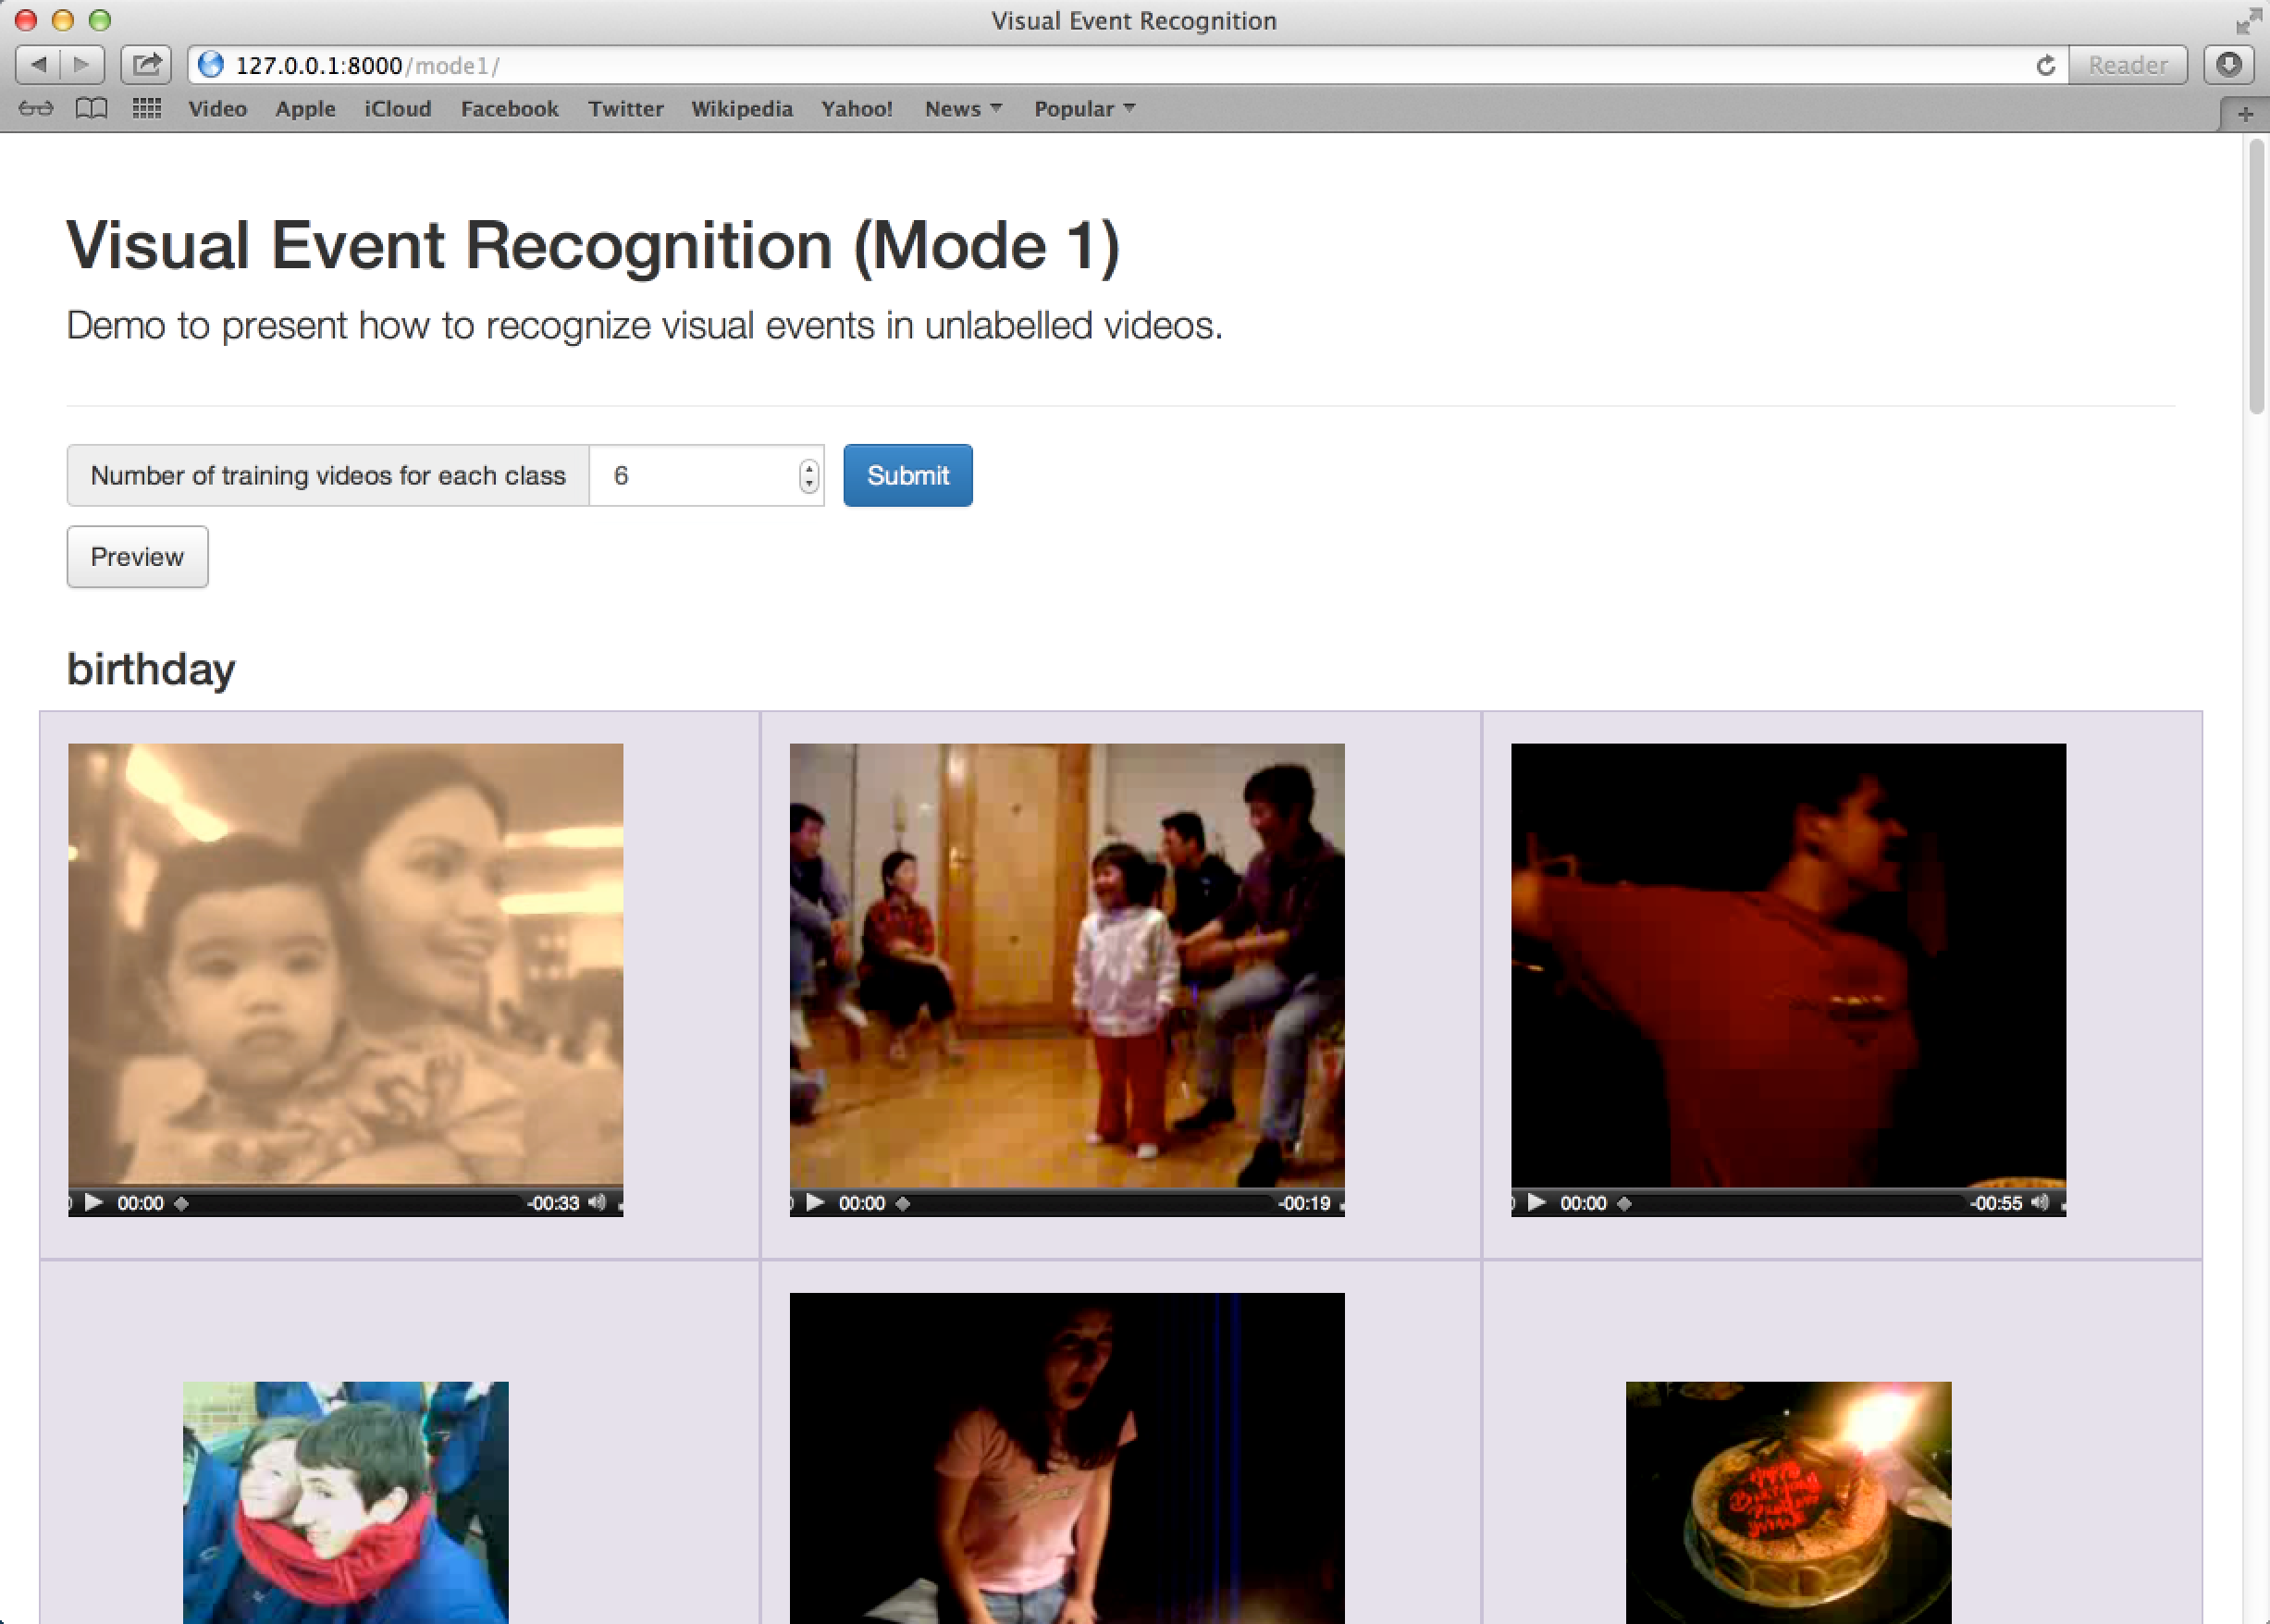
\includegraphics[scale=0.2]{./mode1.png}
\caption{Snapshot of mode 1. In mode 1, the distance matrix of Youtube videos is calculated offline. The user could randomly select the training data and testing data to check the recognition performance.}
\end{figure}

\begin{figure}[!ht]
\centering
	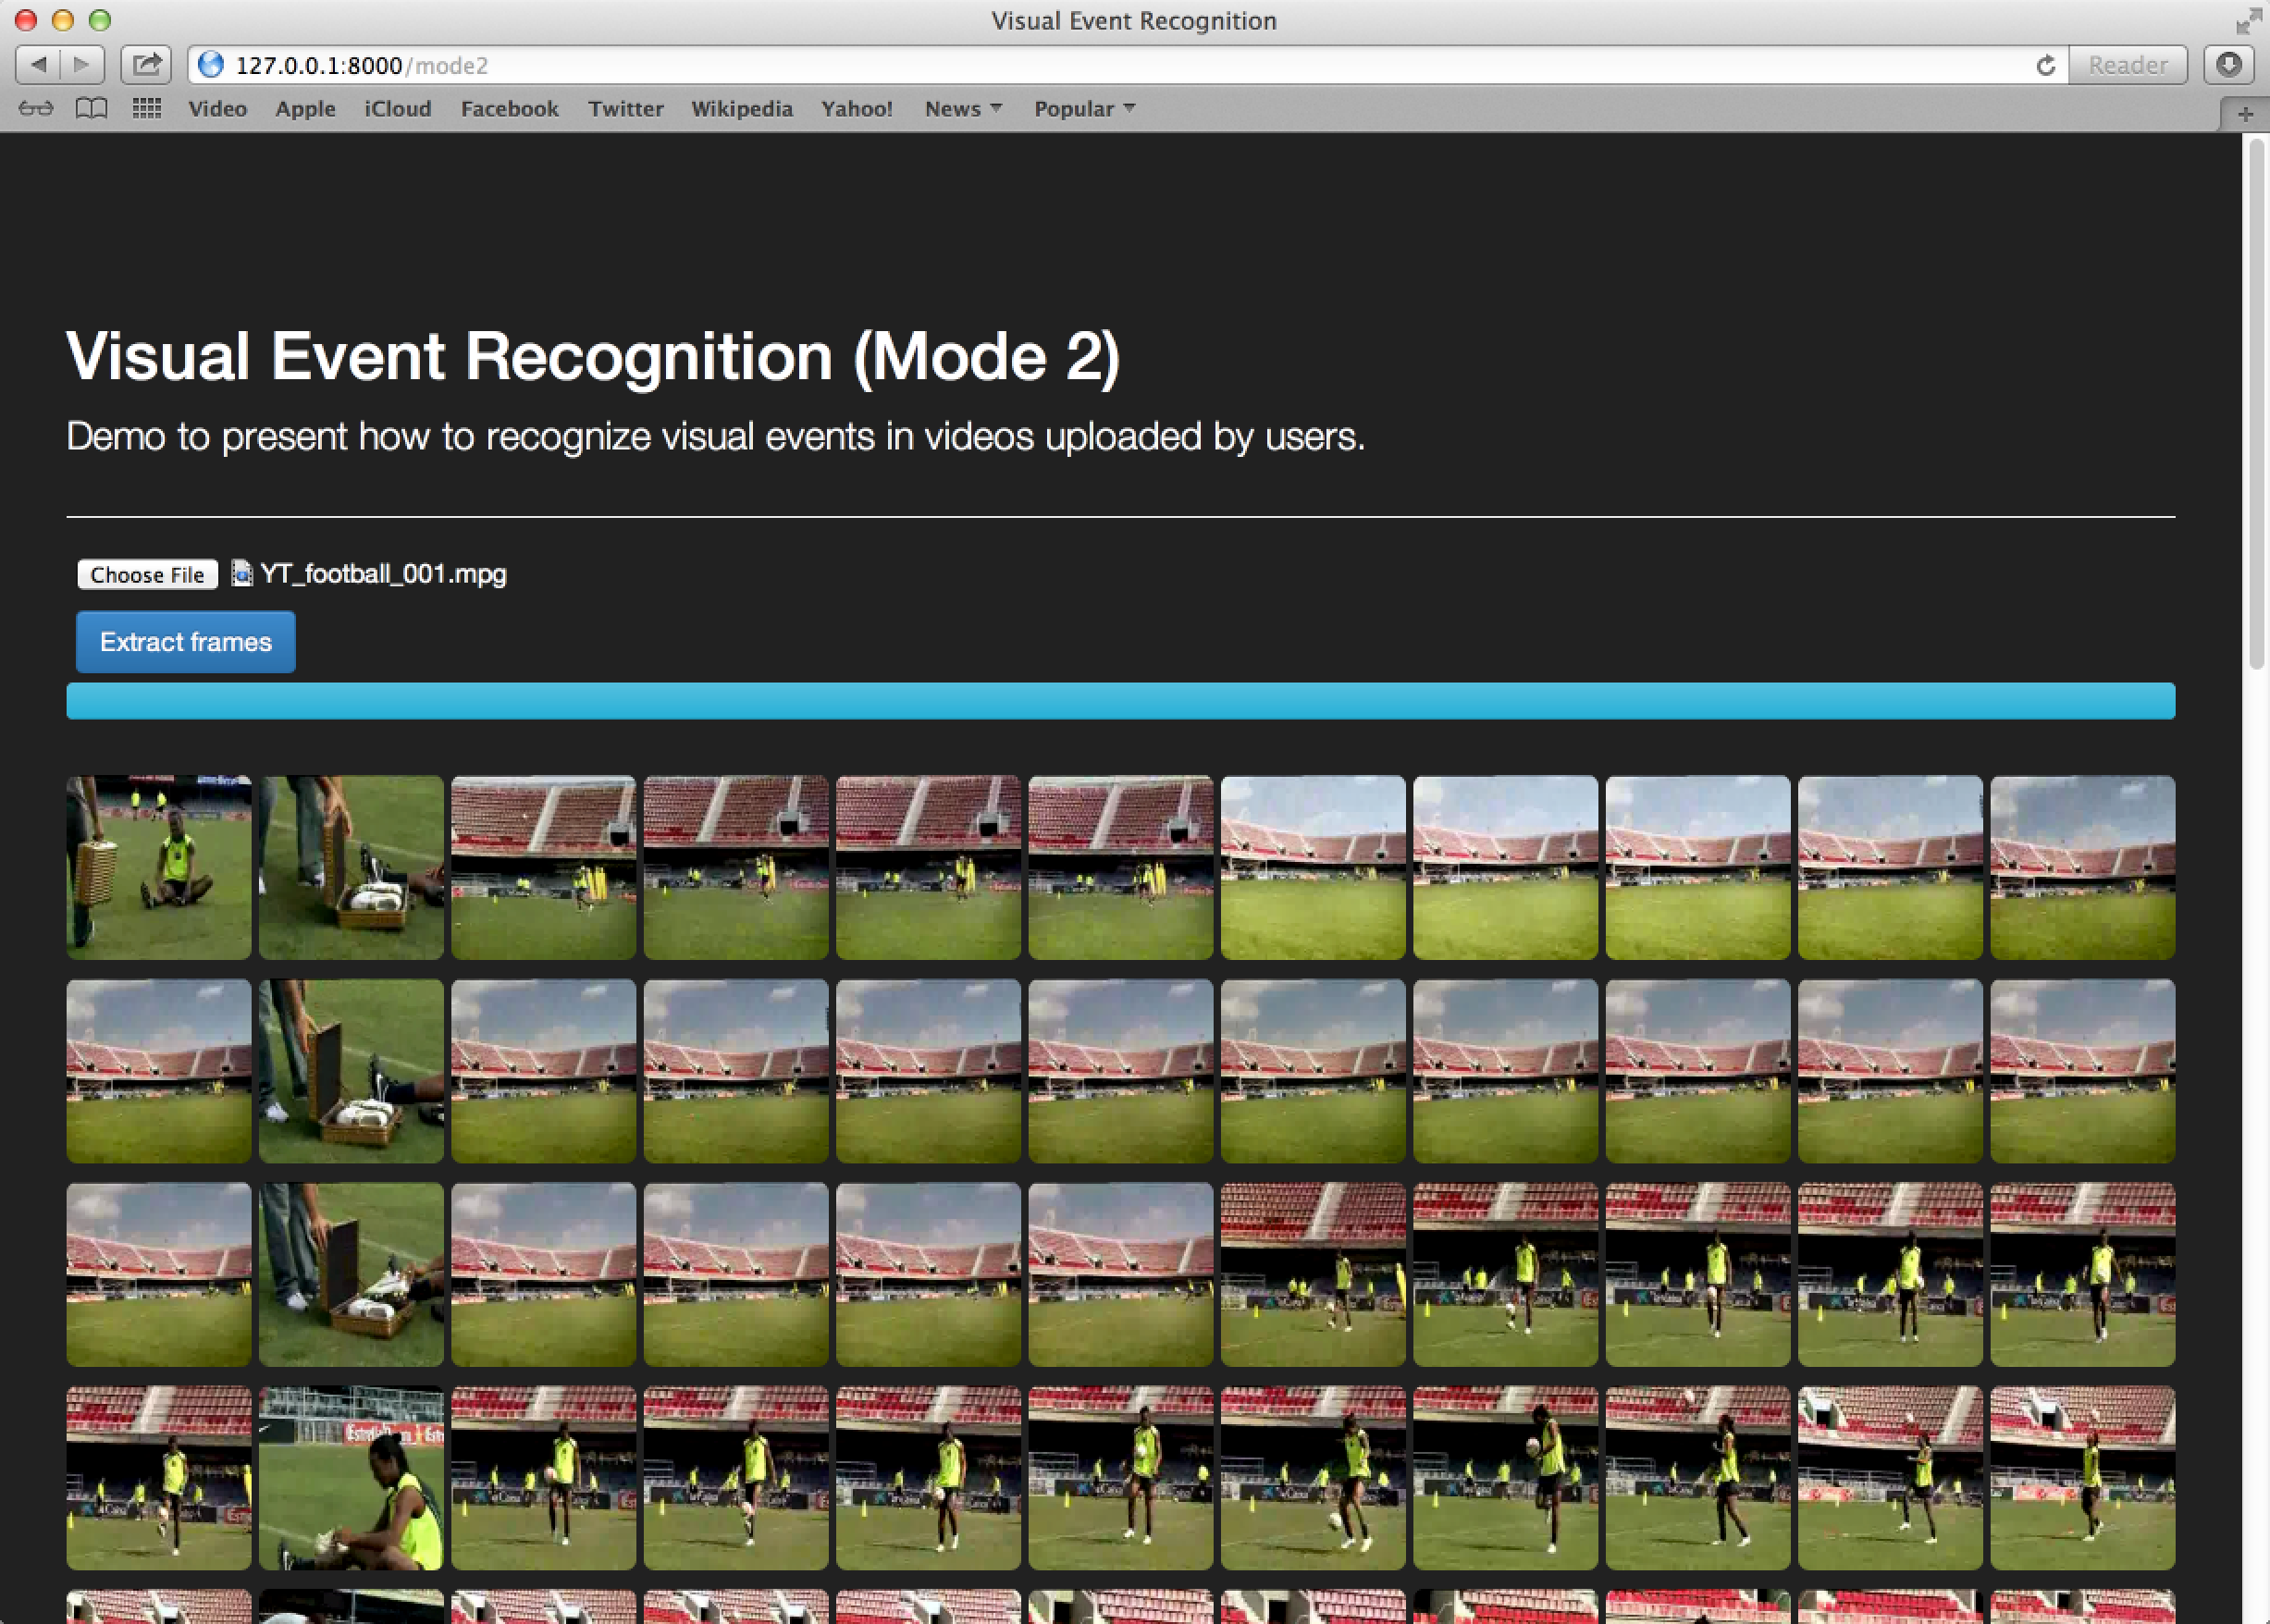
\includegraphics[scale = 0.2]{./mode2.png}
\caption{Snapshot of mode 2. In mode 2, the user could upload a new video and get the label of this video predicted by the underlying recognition system}
\end{figure}

\noindent There are two modes built for two different purposes as shown in Figure 15 and 16. Mode 1 enables the user to randomly select training and testing Youtube videos for recognition. The distance matrix of all Youtube videos used in recognition is calculated offline to save time. The second mode aims to present the user a whole process of recognizing videos. The user could upload a new video and check how this video is recognized from extracting frames, extracting features and building histograms all the way down to calculating distances with training videos and building a classifier for recognition. These two modes shall be able to present this project in a visualizable way. 
% \section{Conclusion}
In conclusion, a recognition system, which recognizes images and videos, has been successfully implemented in various approaches. In image recognition, spatial pyramid is adopted to represents images, and such representations of videos are later on input into SVM and KNN for classification. Moreover, earth mover's distance is incorporated into the calculation of image-to-image distances, and the experiments demonstrate the robustness of EMD. For video recognition, which is the main objective of this project, bag of words and specialized GMMs are used to represent videos compactly, and respective distance calculation methods are employed to measure video-to-video distances. Once the distance calculation is done, it is then converted into gram matrix using four different types of kernel, and SVM is employed to perform classification. Furthermore, four different domain adaptation methods are studied and implemented to improve the performance of classifiers by leveraging labelled samples from other domains. The best result is achieved by Adaptive Multiple Kernel Learning (A-MKL) through selecting two distance matrices smartly, and the recorded mean average precision $61.4\%$ is better than that reported in the studied paper \cite{duan2012visual}. Comprehensive experiments have been conducted on these various approaches, and detailed analysis is also included. Last but not least, a web-based demo system is built to better present the work in this project. \\

\noindent As for future recommendations, there are three suggestions. The first one is to incorporate more types of features including space-time feature and acoustic feature. With more features extracted from videos, the recognition system is expected to be more robust. Secondly, more concept attribute detectors could be employed to represent videos with more attributes. In this way, the produced attribute vector shall possess more discriminative power. Lastly, various domain adaptations could be combined wisely. For instance, Feature Replication could be incorporated into Adaptive Multiple Kernel Learning.  

\newpage
\bibliographystyle{IEEEtranS}
\bibliography{reference}
\end{document}